\documentclass[twoside]{book}

% Packages required by doxygen
\usepackage{calc}
\usepackage{doxygen}
\usepackage{graphicx}
\usepackage[utf8]{inputenc}
\usepackage{makeidx}
\usepackage{multicol}
\usepackage{multirow}
\usepackage{textcomp}
\usepackage[table]{xcolor}

% Font selection
\usepackage[T1]{fontenc}
\usepackage{mathptmx}
\usepackage[scaled=.90]{helvet}
\usepackage{courier}
\usepackage{amssymb}
\usepackage{sectsty}
\renewcommand{\familydefault}{\sfdefault}
\allsectionsfont{%
  \fontseries{bc}\selectfont%
  \color{darkgray}%
}
\renewcommand{\DoxyLabelFont}{%
  \fontseries{bc}\selectfont%
  \color{darkgray}%
}

% Page & text layout
\usepackage{geometry}
\geometry{%
  a4paper,%
  top=2.5cm,%
  bottom=2.5cm,%
  left=2.5cm,%
  right=2.5cm%
}
\tolerance=750
\hfuzz=15pt
\hbadness=750
\setlength{\emergencystretch}{15pt}
\setlength{\parindent}{0cm}
\setlength{\parskip}{0.2cm}
\makeatletter
\renewcommand{\paragraph}{%
  \@startsection{paragraph}{4}{0ex}{-1.0ex}{1.0ex}{%
    \normalfont\normalsize\bfseries\SS@parafont%
  }%
}
\renewcommand{\subparagraph}{%
  \@startsection{subparagraph}{5}{0ex}{-1.0ex}{1.0ex}{%
    \normalfont\normalsize\bfseries\SS@subparafont%
  }%
}
\makeatother

% Headers & footers
\usepackage{fancyhdr}
\pagestyle{fancyplain}
\fancyhead[LE]{\fancyplain{}{\bfseries\thepage}}
\fancyhead[CE]{\fancyplain{}{}}
\fancyhead[RE]{\fancyplain{}{\bfseries\leftmark}}
\fancyhead[LO]{\fancyplain{}{\bfseries\rightmark}}
\fancyhead[CO]{\fancyplain{}{}}
\fancyhead[RO]{\fancyplain{}{\bfseries\thepage}}
\fancyfoot[LE]{\fancyplain{}{}}
\fancyfoot[CE]{\fancyplain{}{}}
\fancyfoot[RE]{\fancyplain{}{\bfseries\scriptsize Generated on Sun May 1 2016 15\-:26\-:28 for “\-Particle\-Panic” by Doxygen }}
\fancyfoot[LO]{\fancyplain{}{\bfseries\scriptsize Generated on Sun May 1 2016 15\-:26\-:28 for “\-Particle\-Panic” by Doxygen }}
\fancyfoot[CO]{\fancyplain{}{}}
\fancyfoot[RO]{\fancyplain{}{}}
\renewcommand{\footrulewidth}{0.4pt}
\renewcommand{\chaptermark}[1]{%
  \markboth{#1}{}%
}
\renewcommand{\sectionmark}[1]{%
  \markright{\thesection\ #1}%
}

% Indices & bibliography
\usepackage{natbib}
\usepackage[titles]{tocloft}
\setcounter{tocdepth}{3}
\setcounter{secnumdepth}{5}
\makeindex

% Hyperlinks (required, but should be loaded last)
\usepackage{ifpdf}
\ifpdf
  \usepackage[pdftex,pagebackref=true]{hyperref}
\else
  \usepackage[ps2pdf,pagebackref=true]{hyperref}
\fi
\hypersetup{%
  colorlinks=true,%
  linkcolor=blue,%
  citecolor=blue,%
  unicode%
}

% Custom commands
\newcommand{\clearemptydoublepage}{%
  \newpage{\pagestyle{empty}\cleardoublepage}%
}


%===== C O N T E N T S =====

\begin{document}

% Titlepage & ToC
\hypersetup{pageanchor=false}
\pagenumbering{roman}
\begin{titlepage}
\vspace*{7cm}
\begin{center}%
{\Large “\-Particle\-Panic” }\\
\vspace*{1cm}
{\large Generated by Doxygen 1.8.5}\\
\vspace*{0.5cm}
{\small Sun May 1 2016 15:26:28}\\
\end{center}
\end{titlepage}
\clearemptydoublepage
\tableofcontents
\clearemptydoublepage
\pagenumbering{arabic}
\hypersetup{pageanchor=true}

%--- Begin generated contents ---
\chapter{Hierarchical Index}
\section{Class Hierarchy}
This inheritance list is sorted roughly, but not completely, alphabetically\-:\begin{DoxyCompactList}
\item \contentsline{section}{Command}{\pageref{classCommand}}{}
\begin{DoxyCompactList}
\item \contentsline{section}{Clear\-World}{\pageref{classClearWorld}}{}
\item \contentsline{section}{Mouse\-Drag}{\pageref{classMouseDrag}}{}
\item \contentsline{section}{Mouse\-Drag\-End}{\pageref{classMouseDragEnd}}{}
\item \contentsline{section}{Mouse\-Draw}{\pageref{classMouseDraw}}{}
\item \contentsline{section}{Mouse\-Erase}{\pageref{classMouseErase}}{}
\item \contentsline{section}{Resize\-World}{\pageref{classResizeWorld}}{}
\item \contentsline{section}{Select\-Dragged\-Particles}{\pageref{classSelectDraggedParticles}}{}
\item \contentsline{section}{Set3\-D}{\pageref{classSet3D}}{}
\end{DoxyCompactList}
\item \contentsline{section}{Marching\-Algorithms}{\pageref{classMarchingAlgorithms}}{}
\item \contentsline{section}{Mat3}{\pageref{classMat3}}{}
\item \contentsline{section}{Particle}{\pageref{classParticle}}{}
\item \contentsline{section}{Particle\-Properties}{\pageref{classParticleProperties}}{}
\item \contentsline{section}{Particle\-:\-:spring}{\pageref{structParticle_1_1spring}}{}
\item \contentsline{section}{Toolbar}{\pageref{classToolbar}}{}
\item \contentsline{section}{Vec3}{\pageref{classVec3}}{}
\item \contentsline{section}{World}{\pageref{classWorld}}{}
\end{DoxyCompactList}

\chapter{Class Index}
\section{Class List}
Here are the classes, structs, unions and interfaces with brief descriptions\-:\begin{DoxyCompactList}
\item\contentsline{section}{\hyperlink{classClearWorld}{Clear\-World} }{\pageref{classClearWorld}}{}
\item\contentsline{section}{\hyperlink{classCommand}{Command} }{\pageref{classCommand}}{}
\item\contentsline{section}{\hyperlink{classMarchingAlgorithms}{Marching\-Algorithms} }{\pageref{classMarchingAlgorithms}}{}
\item\contentsline{section}{\hyperlink{classMat3}{Mat3} }{\pageref{classMat3}}{}
\item\contentsline{section}{\hyperlink{classMouseDrag}{Mouse\-Drag} }{\pageref{classMouseDrag}}{}
\item\contentsline{section}{\hyperlink{classMouseDragEnd}{Mouse\-Drag\-End} }{\pageref{classMouseDragEnd}}{}
\item\contentsline{section}{\hyperlink{classMouseDraw}{Mouse\-Draw} }{\pageref{classMouseDraw}}{}
\item\contentsline{section}{\hyperlink{classMouseErase}{Mouse\-Erase} }{\pageref{classMouseErase}}{}
\item\contentsline{section}{\hyperlink{classParticle}{Particle} }{\pageref{classParticle}}{}
\item\contentsline{section}{\hyperlink{classParticleProperties}{Particle\-Properties} }{\pageref{classParticleProperties}}{}
\item\contentsline{section}{\hyperlink{classResizeWorld}{Resize\-World} }{\pageref{classResizeWorld}}{}
\item\contentsline{section}{\hyperlink{classSelectDraggedParticles}{Select\-Dragged\-Particles} }{\pageref{classSelectDraggedParticles}}{}
\item\contentsline{section}{\hyperlink{classSet3D}{Set3\-D} }{\pageref{classSet3D}}{}
\item\contentsline{section}{\hyperlink{structParticle_1_1spring}{Particle\-::spring} }{\pageref{structParticle_1_1spring}}{}
\item\contentsline{section}{\hyperlink{classToolbar}{Toolbar} }{\pageref{classToolbar}}{}
\item\contentsline{section}{\hyperlink{classVec3}{Vec3} }{\pageref{classVec3}}{}
\item\contentsline{section}{\hyperlink{classWorld}{World} \\*The Scene class }{\pageref{classWorld}}{}
\end{DoxyCompactList}

\chapter{File Index}
\section{File List}
Here is a list of all documented files with brief descriptions\-:\begin{DoxyCompactList}
\item\contentsline{section}{include/\hyperlink{Commands_8h}{Commands.\-h} \\*\hyperlink{classCommand}{Command} objects to be executed inside timer\-Callback in main. The purpose of this is to make sure the commands are not executed in the middle of update() when outside the timer }{\pageref{Commands_8h}}{}
\item\contentsline{section}{include/\hyperlink{MarchingAlgorithms_8h}{Marching\-Algorithms.\-h} \\*Contains the marching cube / square triangle vectors and algorithms to draw and create them }{\pageref{MarchingAlgorithms_8h}}{}
\item\contentsline{section}{include/\hyperlink{Mat3_8h}{Mat3.\-h} \\*Object needed to rotate particles in 3\-D mode }{\pageref{Mat3_8h}}{}
\item\contentsline{section}{include/\hyperlink{Particle_8h}{Particle.\-h} \\*\hyperlink{classParticle}{Particle} class that includes all attributes of the particle }{\pageref{Particle_8h}}{}
\item\contentsline{section}{include/\hyperlink{ParticleProperties_8h}{Particle\-Properties.\-h} \\*Properties of a particle type. Each particle has a pointer to such a class }{\pageref{ParticleProperties_8h}}{}
\item\contentsline{section}{include/\hyperlink{Toolbar_8h}{Toolbar.\-h} \\*G\-U\-I implementation from scratch, includes draw and input interaction }{\pageref{Toolbar_8h}}{}
\item\contentsline{section}{include/\hyperlink{Vec3_8h}{Vec3.\-h} \\*Encapsulates a 3d Point / Vector object. Homogenous is not needed }{\pageref{Vec3_8h}}{}
\item\contentsline{section}{include/\hyperlink{World_8h}{World.\-h} \\*All particles and methods to draw and update them }{\pageref{World_8h}}{}
\item\contentsline{section}{libraries/cegui/include/\-C\-E\-G\-U\-I/{\bfseries Config.\-h} }{\pageref{Config_8h}}{}
\item\contentsline{section}{libraries/cegui/include/\-C\-E\-G\-U\-I/{\bfseries Module\-Config.\-h} }{\pageref{ModuleConfig_8h}}{}
\item\contentsline{section}{libraries/cegui/include/\-C\-E\-G\-U\-I/{\bfseries Version.\-h} }{\pageref{Version_8h}}{}
\end{DoxyCompactList}

\chapter{Class Documentation}
\hypertarget{classClearWorld}{\section{Clear\-World Class Reference}
\label{classClearWorld}\index{Clear\-World@{Clear\-World}}
}
Inheritance diagram for Clear\-World\-:\begin{figure}[H]
\begin{center}
\leavevmode
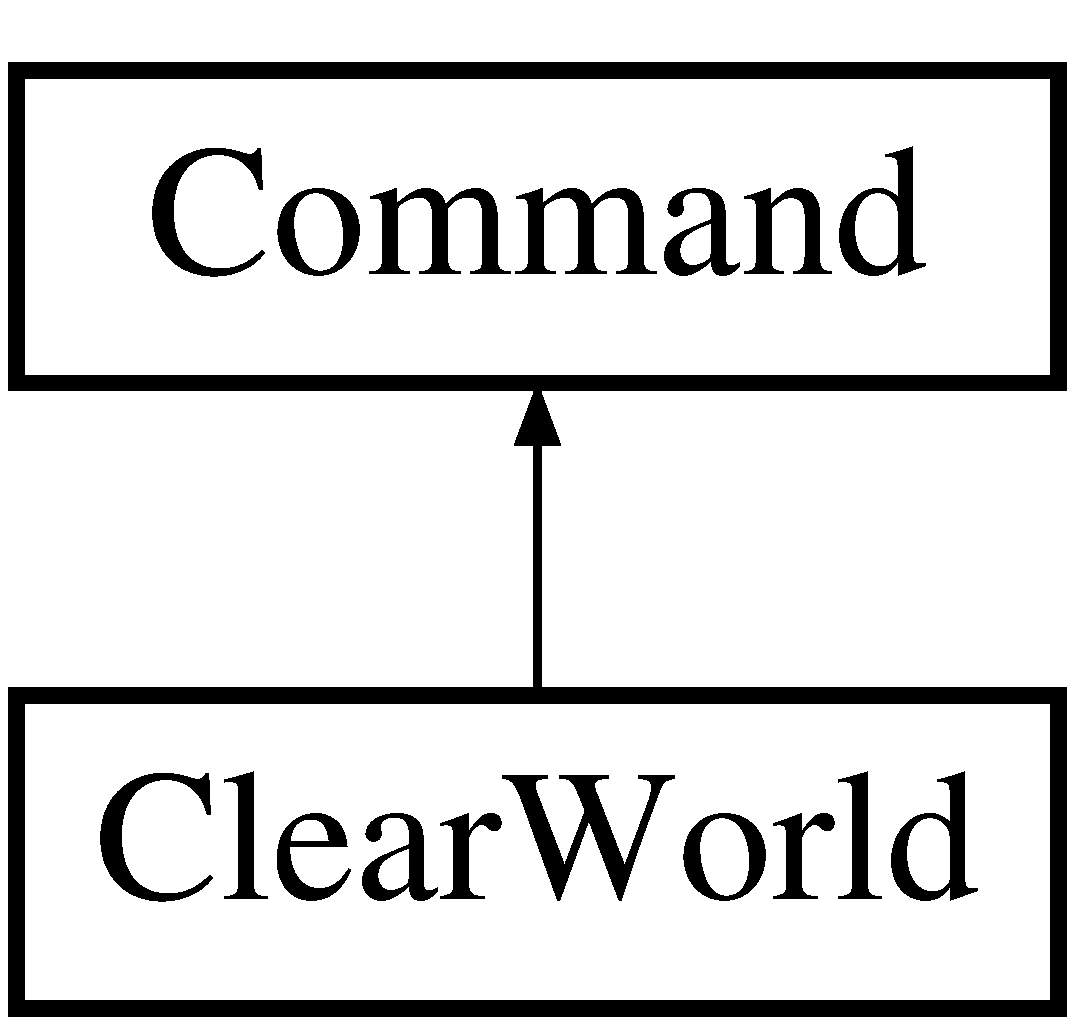
\includegraphics[height=2.000000cm]{classClearWorld}
\end{center}
\end{figure}
\subsection*{Public Member Functions}
\begin{DoxyCompactItemize}
\item 
\hypertarget{classClearWorld_a41ad61c93dc9eaafe3285a91a9adb637}{void {\bfseries execute} ()}\label{classClearWorld_a41ad61c93dc9eaafe3285a91a9adb637}

\end{DoxyCompactItemize}
\subsection*{Additional Inherited Members}


The documentation for this class was generated from the following file\-:\begin{DoxyCompactItemize}
\item 
include/\hyperlink{Commands_8h}{Commands.\-h}\end{DoxyCompactItemize}

\hypertarget{classCommand}{\section{Command Class Reference}
\label{classCommand}\index{Command@{Command}}
}
Inheritance diagram for Command\-:\begin{figure}[H]
\begin{center}
\leavevmode
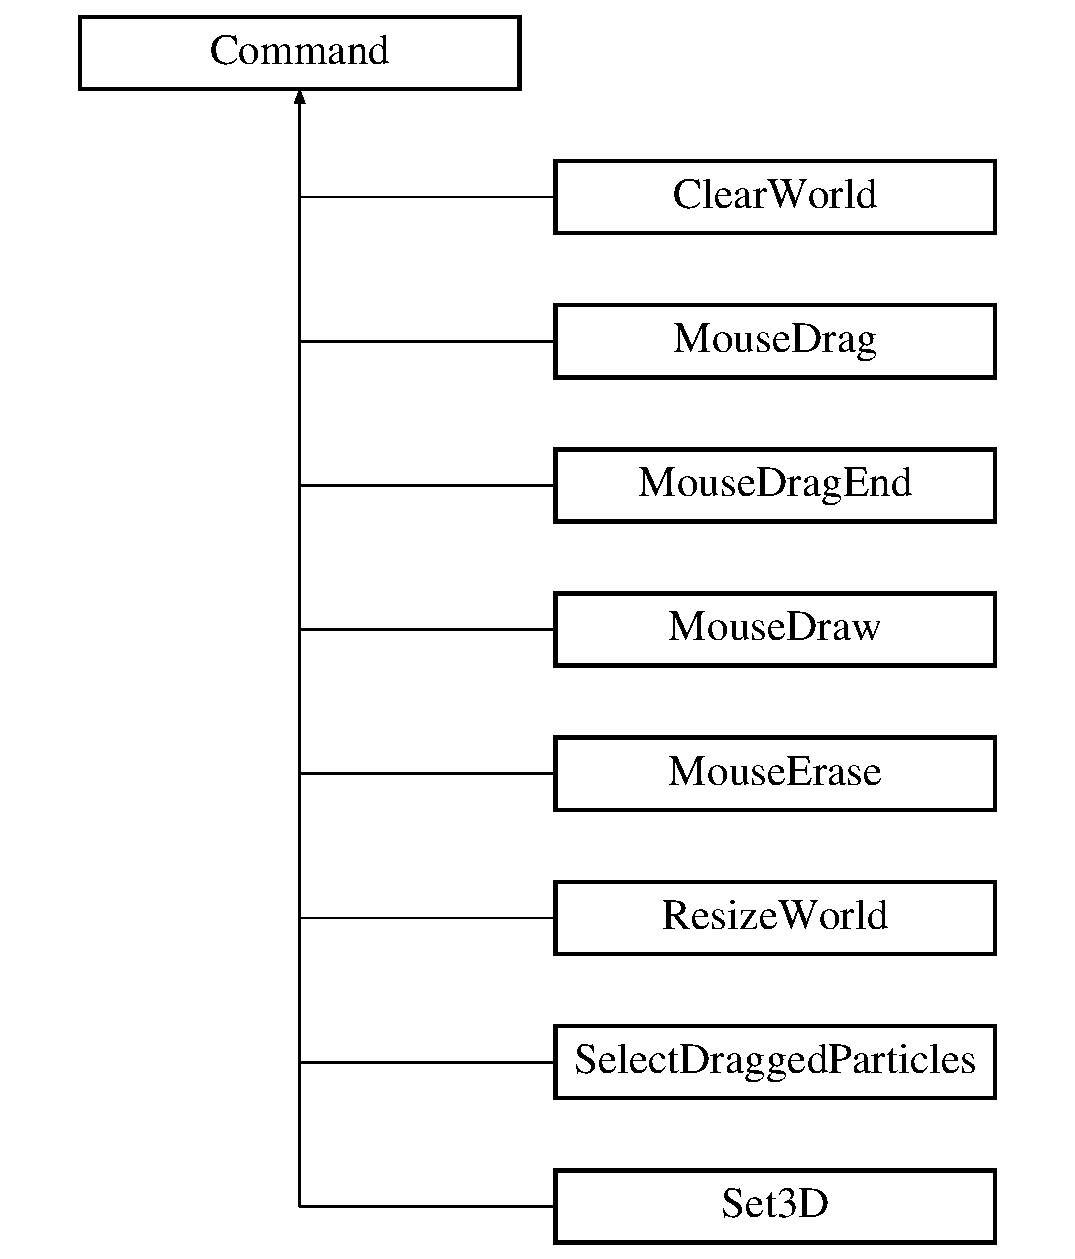
\includegraphics[height=9.000000cm]{classCommand}
\end{center}
\end{figure}
\subsection*{Public Member Functions}
\begin{DoxyCompactItemize}
\item 
\hypertarget{classCommand_a6fd7d9bd8df8bfc881e4d6c7cd1878b7}{virtual void {\bfseries execute} ()=0}\label{classCommand_a6fd7d9bd8df8bfc881e4d6c7cd1878b7}

\item 
\hypertarget{classCommand_aca6e0ee5ee282b6e751e615cc6d42c44}{void {\bfseries set\-World} (\hyperlink{classWorld}{World} $\ast$\-\_\-world)}\label{classCommand_aca6e0ee5ee282b6e751e615cc6d42c44}

\end{DoxyCompactItemize}
\subsection*{Protected Attributes}
\begin{DoxyCompactItemize}
\item 
\hypertarget{classCommand_af7d2460e597be6d61005521563d974b5}{\hyperlink{classWorld}{World} $\ast$ {\bfseries m\-\_\-world}}\label{classCommand_af7d2460e597be6d61005521563d974b5}

\end{DoxyCompactItemize}


The documentation for this class was generated from the following file\-:\begin{DoxyCompactItemize}
\item 
include/\hyperlink{Commands_8h}{Commands.\-h}\end{DoxyCompactItemize}

\hypertarget{classMarchingAlgorithms}{\section{Marching\-Algorithms Class Reference}
\label{classMarchingAlgorithms}\index{Marching\-Algorithms@{Marching\-Algorithms}}
}
\subsection*{Public Member Functions}
\begin{DoxyCompactItemize}
\item 
\hyperlink{classMarchingAlgorithms_af884d18ba13d54b68c3148d859219a31}{Marching\-Algorithms} (const float \-\_\-render2d\-Threshold, const float \-\_\-render3d\-Threshold, const float \-\_\-squaresize, const float \-\_\-renderresolution, const float \-\_\-render3dresolution, const float \-\_\-halfwidth, const float \-\_\-halfheight, const float \-\_\-snapshotmultiplier)
\begin{DoxyCompactList}\small\item\em \hyperlink{classMarchingAlgorithms}{Marching\-Algorithms} constructor for \hyperlink{classMarchingAlgorithms}{Marching\-Algorithms}. \end{DoxyCompactList}\item 
void \hyperlink{classMarchingAlgorithms_a0b6fb536f84f8cd573110c8568d8978f}{calculate\-Marching\-Squares} (const std\-::vector$<$ std\-::vector$<$ float $>$$>$ render\-Grid, const \hyperlink{classParticleProperties}{Particle\-Properties} p, const bool inner)
\begin{DoxyCompactList}\small\item\em calculate\-Marching\-Squares fills m\-\_\-realtime2\-D\-Triangles full of triangle verticies and colors \end{DoxyCompactList}\item 
void \hyperlink{classMarchingAlgorithms_ad3ea84f528558c3057eb71598ace118a}{calculate\-Marching\-Cubes} (const std\-::vector$<$ std\-::vector$<$ std\-::vector$<$ float $>$$>$$>$ render\-Grid, const \hyperlink{classParticleProperties}{Particle\-Properties} p)
\begin{DoxyCompactList}\small\item\em calculate\-Marching\-Cubes fills m\-\_\-snapshot3\-D\-Triangles or m\-\_\-realtime3\-D\-Triangles with triangle verticies and colors \end{DoxyCompactList}\item 
\hyperlink{classVec3}{Vec3} \hyperlink{classMarchingAlgorithms_afe2a91dcd2b7948e0980acd2f2a73322}{Vertex\-Interp} (const \hyperlink{classVec3}{Vec3} p1, const \hyperlink{classVec3}{Vec3} p2, const float valp1, const float valp2)
\begin{DoxyCompactList}\small\item\em Vertex\-Interp calculates the position between two points depending on the floats at either point. \end{DoxyCompactList}\item 
\hypertarget{classMarchingAlgorithms_ad3b6c48ca79f9e91837a0760d6683674}{void \hyperlink{classMarchingAlgorithms_ad3b6c48ca79f9e91837a0760d6683674}{draw2\-D\-Realtime} ()}\label{classMarchingAlgorithms_ad3b6c48ca79f9e91837a0760d6683674}

\begin{DoxyCompactList}\small\item\em draw2\-D\-Realtime draws the m\-\_\-realtime2\-D\-Triangle Vec3s using Open\-G\-L gl\-Begin(\-G\-L\-\_\-\-T\-R\-I\-A\-N\-G\-L\-E\-S) \end{DoxyCompactList}\item 
\hypertarget{classMarchingAlgorithms_aceccb617c45738f065a38634a8ddb896}{void \hyperlink{classMarchingAlgorithms_aceccb617c45738f065a38634a8ddb896}{draw3\-D\-Realtime} ()}\label{classMarchingAlgorithms_aceccb617c45738f065a38634a8ddb896}

\begin{DoxyCompactList}\small\item\em draw3\-D\-Realtime draws the m\-\_\-realtime3\-D\-Triangle Vec3s using Open\-G\-L gl\-Begin(\-G\-L\-\_\-\-T\-R\-I\-A\-N\-G\-L\-E\-S) (calculates normals as well) \end{DoxyCompactList}\item 
\hypertarget{classMarchingAlgorithms_a53c874fc236e6a1da1c26f6c0dd9747a}{void \hyperlink{classMarchingAlgorithms_a53c874fc236e6a1da1c26f6c0dd9747a}{draw3\-D\-Snapshot} ()}\label{classMarchingAlgorithms_a53c874fc236e6a1da1c26f6c0dd9747a}

\begin{DoxyCompactList}\small\item\em draw3\-D\-Snapshot draws the m\-\_\-snapshot3\-D\-Triangle Vec3s using Open\-G\-L gl\-Begin(\-G\-L\-\_\-\-T\-R\-I\-A\-N\-G\-L\-E\-S) (calculates normals as well) \end{DoxyCompactList}\item 
int \hyperlink{classMarchingAlgorithms_a36c86931558ec0de770baf06f6a8e2a5}{get\-Snapshot\-Mode} ()
\begin{DoxyCompactList}\small\item\em get\-Snapshot\-Mode returns the snapshot mode integer \end{DoxyCompactList}\item 
void \hyperlink{classMarchingAlgorithms_a9fafe791d5a20410bce4200709fa666a}{set\-Snapshot\-Mode} (const int \-\_\-s)
\begin{DoxyCompactList}\small\item\em set\-Snapshot\-Mode sets the m\-\_\-snapshot\-Mode that shows where in the snapshot process we are \end{DoxyCompactList}\item 
void \hyperlink{classMarchingAlgorithms_a4b80a9c0f5d814ed1d931655b3472c38}{set\-Square\-Size} (const float ss)
\begin{DoxyCompactList}\small\item\em set\-Square\-Size sets m\-\_\-squaresize which is the width/height of the square in the rendergrid \end{DoxyCompactList}\item 
\hypertarget{classMarchingAlgorithms_a2c340f6b3e3fc8ce8c06d7df8dfc3d1c}{void \hyperlink{classMarchingAlgorithms_a2c340f6b3e3fc8ce8c06d7df8dfc3d1c}{toggle3\-D\-Resolution} ()}\label{classMarchingAlgorithms_a2c340f6b3e3fc8ce8c06d7df8dfc3d1c}

\begin{DoxyCompactList}\small\item\em toggle3\-D\-Resolution either multiplies or divides the 3d render resolution by 6 -\/ used for high poly snapshot \end{DoxyCompactList}\item 
\hypertarget{classMarchingAlgorithms_a55306a1801044ba00de5211f2408ad92}{void \hyperlink{classMarchingAlgorithms_a55306a1801044ba00de5211f2408ad92}{clear\-Realtime2\-D\-Triangles} ()}\label{classMarchingAlgorithms_a55306a1801044ba00de5211f2408ad92}

\begin{DoxyCompactList}\small\item\em clear\-Realtime2\-D\-Triangles clears the std\-::vector m\-\_\-realtime2\-D\-Triangles \end{DoxyCompactList}\item 
\hypertarget{classMarchingAlgorithms_a15e0be9c959ad5b35cc92f91546af3d2}{void \hyperlink{classMarchingAlgorithms_a15e0be9c959ad5b35cc92f91546af3d2}{clear\-Realtime3\-D\-Triangles} ()}\label{classMarchingAlgorithms_a15e0be9c959ad5b35cc92f91546af3d2}

\begin{DoxyCompactList}\small\item\em clear\-Realtime3\-D\-Triangles clears the std\-::vector m\-\_\-realtime3\-D\-Triangles \end{DoxyCompactList}\item 
\hypertarget{classMarchingAlgorithms_afb08a29dcb96256be0469b64fde74b05}{void \hyperlink{classMarchingAlgorithms_afb08a29dcb96256be0469b64fde74b05}{clear\-Snapshot3\-D\-Triangles} ()}\label{classMarchingAlgorithms_afb08a29dcb96256be0469b64fde74b05}

\begin{DoxyCompactList}\small\item\em clear\-Snapshot3\-D\-Triangles clears the 4d std\-::vector m\-\_\-realtime3\-D\-Triangles and resizes them to the 3d render width, height and depth. \end{DoxyCompactList}\item 
\hypertarget{classMarchingAlgorithms_a09372b6314026f6045db3b51bc6b8782}{void \hyperlink{classMarchingAlgorithms_a09372b6314026f6045db3b51bc6b8782}{increase2\-D\-Resolution} ()}\label{classMarchingAlgorithms_a09372b6314026f6045db3b51bc6b8782}

\begin{DoxyCompactList}\small\item\em increase2\-D\-Resolution increases the 2\-D marching squares resolution by 1 \end{DoxyCompactList}\item 
\hypertarget{classMarchingAlgorithms_af72442c4c16cb90bf339b63e0a0ff803}{void \hyperlink{classMarchingAlgorithms_af72442c4c16cb90bf339b63e0a0ff803}{decrease2\-D\-Resolution} ()}\label{classMarchingAlgorithms_af72442c4c16cb90bf339b63e0a0ff803}

\begin{DoxyCompactList}\small\item\em decrease2\-D\-Resolution decreases the 2\-D marching squares resolution by 1 (but not when it is 1) \end{DoxyCompactList}\end{DoxyCompactItemize}


\subsection{Constructor \& Destructor Documentation}
\hypertarget{classMarchingAlgorithms_af884d18ba13d54b68c3148d859219a31}{\index{Marching\-Algorithms@{Marching\-Algorithms}!Marching\-Algorithms@{Marching\-Algorithms}}
\index{Marching\-Algorithms@{Marching\-Algorithms}!MarchingAlgorithms@{Marching\-Algorithms}}
\subsubsection[{Marching\-Algorithms}]{\setlength{\rightskip}{0pt plus 5cm}Marching\-Algorithms\-::\-Marching\-Algorithms (
\begin{DoxyParamCaption}
\item[{const float}]{\-\_\-render2d\-Threshold, }
\item[{const float}]{\-\_\-render3d\-Threshold, }
\item[{const float}]{\-\_\-squaresize, }
\item[{const float}]{\-\_\-renderresolution, }
\item[{const float}]{\-\_\-render3dresolution, }
\item[{const float}]{\-\_\-halfwidth, }
\item[{const float}]{\-\_\-halfheight, }
\item[{const float}]{\-\_\-snapshotmultiplier}
\end{DoxyParamCaption}
)\hspace{0.3cm}{\ttfamily [inline]}}}\label{classMarchingAlgorithms_af884d18ba13d54b68c3148d859219a31}


\hyperlink{classMarchingAlgorithms}{Marching\-Algorithms} constructor for \hyperlink{classMarchingAlgorithms}{Marching\-Algorithms}. 


\begin{DoxyParams}[1]{Parameters}
\mbox{\tt in}  & {\em \-\_\-render2d\-Threshold} & sets the renderthreshold for which to draw the marching squares with \\
\hline
\mbox{\tt in}  & {\em \-\_\-render3d\-Threshold} & sets the isolevel for which to draw the marching cubes with \\
\hline
\mbox{\tt in}  & {\em \-\_\-squaresize} & sets the width/height of the square in the rendergrid \\
\hline
\mbox{\tt in}  & {\em \-\_\-renderresolution} & sets the renderresolution for the 2d marching squares \\
\hline
\mbox{\tt in}  & {\em \-\_\-render3dresolution} & sets the renderresolution for the 3d marching squares \\
\hline
\mbox{\tt in}  & {\em \-\_\-halfwidth} & sets the halfwidth -\/ half the screen's width in opengl's coordinate system \\
\hline
\mbox{\tt in}  & {\em \-\_\-halfheight} & sets the halfheight -\/ half the screen's height in opengl's coordinate system \\
\hline
\end{DoxyParams}


\subsection{Member Function Documentation}
\hypertarget{classMarchingAlgorithms_ad3ea84f528558c3057eb71598ace118a}{\index{Marching\-Algorithms@{Marching\-Algorithms}!calculate\-Marching\-Cubes@{calculate\-Marching\-Cubes}}
\index{calculate\-Marching\-Cubes@{calculate\-Marching\-Cubes}!MarchingAlgorithms@{Marching\-Algorithms}}
\subsubsection[{calculate\-Marching\-Cubes}]{\setlength{\rightskip}{0pt plus 5cm}void Marching\-Algorithms\-::calculate\-Marching\-Cubes (
\begin{DoxyParamCaption}
\item[{const std\-::vector$<$ std\-::vector$<$ std\-::vector$<$ float $>$$>$$>$}]{render\-Grid, }
\item[{const {\bf Particle\-Properties}}]{p}
\end{DoxyParamCaption}
)}}\label{classMarchingAlgorithms_ad3ea84f528558c3057eb71598ace118a}


calculate\-Marching\-Cubes fills m\-\_\-snapshot3\-D\-Triangles or m\-\_\-realtime3\-D\-Triangles with triangle verticies and colors 


\begin{DoxyParams}[1]{Parameters}
\mbox{\tt in}  & {\em \-\_\-render\-Grid} & the 3d rendergrid containing the metaball floats \\
\hline
\mbox{\tt in}  & {\em \-\_\-p} & particle properties -\/ used for the colour attributes \\
\hline
\end{DoxyParams}
\hypertarget{classMarchingAlgorithms_a0b6fb536f84f8cd573110c8568d8978f}{\index{Marching\-Algorithms@{Marching\-Algorithms}!calculate\-Marching\-Squares@{calculate\-Marching\-Squares}}
\index{calculate\-Marching\-Squares@{calculate\-Marching\-Squares}!MarchingAlgorithms@{Marching\-Algorithms}}
\subsubsection[{calculate\-Marching\-Squares}]{\setlength{\rightskip}{0pt plus 5cm}void Marching\-Algorithms\-::calculate\-Marching\-Squares (
\begin{DoxyParamCaption}
\item[{const std\-::vector$<$ std\-::vector$<$ float $>$$>$}]{render\-Grid, }
\item[{const {\bf Particle\-Properties}}]{p, }
\item[{const bool}]{inner}
\end{DoxyParamCaption}
)}}\label{classMarchingAlgorithms_a0b6fb536f84f8cd573110c8568d8978f}


calculate\-Marching\-Squares fills m\-\_\-realtime2\-D\-Triangles full of triangle verticies and colors 


\begin{DoxyParams}[1]{Parameters}
\mbox{\tt in}  & {\em \-\_\-render\-Grid} & the 2d rendergrid containing the metaball floats \\
\hline
\mbox{\tt in}  & {\em \-\_\-p} & particle properties -\/ used for the colour attributes \\
\hline
\mbox{\tt in}  & {\em \-\_\-inner} & whether to increase the threshold for the outer rim effect for the liquid \\
\hline
\end{DoxyParams}
\hypertarget{classMarchingAlgorithms_a36c86931558ec0de770baf06f6a8e2a5}{\index{Marching\-Algorithms@{Marching\-Algorithms}!get\-Snapshot\-Mode@{get\-Snapshot\-Mode}}
\index{get\-Snapshot\-Mode@{get\-Snapshot\-Mode}!MarchingAlgorithms@{Marching\-Algorithms}}
\subsubsection[{get\-Snapshot\-Mode}]{\setlength{\rightskip}{0pt plus 5cm}int Marching\-Algorithms\-::get\-Snapshot\-Mode (
\begin{DoxyParamCaption}
{}
\end{DoxyParamCaption}
)}}\label{classMarchingAlgorithms_a36c86931558ec0de770baf06f6a8e2a5}


get\-Snapshot\-Mode returns the snapshot mode integer 

\begin{DoxyReturn}{Returns}
returns m\-\_\-snapshot\-Mode 
\end{DoxyReturn}
\hypertarget{classMarchingAlgorithms_a9fafe791d5a20410bce4200709fa666a}{\index{Marching\-Algorithms@{Marching\-Algorithms}!set\-Snapshot\-Mode@{set\-Snapshot\-Mode}}
\index{set\-Snapshot\-Mode@{set\-Snapshot\-Mode}!MarchingAlgorithms@{Marching\-Algorithms}}
\subsubsection[{set\-Snapshot\-Mode}]{\setlength{\rightskip}{0pt plus 5cm}void Marching\-Algorithms\-::set\-Snapshot\-Mode (
\begin{DoxyParamCaption}
\item[{const int}]{\-\_\-s}
\end{DoxyParamCaption}
)}}\label{classMarchingAlgorithms_a9fafe791d5a20410bce4200709fa666a}


set\-Snapshot\-Mode sets the m\-\_\-snapshot\-Mode that shows where in the snapshot process we are 


\begin{DoxyParams}{Parameters}
{\em \-\_\-s} & the integer to set m\-\_\-snapshot\-Mode to \\
\hline
\end{DoxyParams}
\hypertarget{classMarchingAlgorithms_a4b80a9c0f5d814ed1d931655b3472c38}{\index{Marching\-Algorithms@{Marching\-Algorithms}!set\-Square\-Size@{set\-Square\-Size}}
\index{set\-Square\-Size@{set\-Square\-Size}!MarchingAlgorithms@{Marching\-Algorithms}}
\subsubsection[{set\-Square\-Size}]{\setlength{\rightskip}{0pt plus 5cm}void Marching\-Algorithms\-::set\-Square\-Size (
\begin{DoxyParamCaption}
\item[{const float}]{ss}
\end{DoxyParamCaption}
)}}\label{classMarchingAlgorithms_a4b80a9c0f5d814ed1d931655b3472c38}


set\-Square\-Size sets m\-\_\-squaresize which is the width/height of the square in the rendergrid 


\begin{DoxyParams}{Parameters}
{\em ss} & the float to set m\-\_\-squaresize to \\
\hline
\end{DoxyParams}
\hypertarget{classMarchingAlgorithms_afe2a91dcd2b7948e0980acd2f2a73322}{\index{Marching\-Algorithms@{Marching\-Algorithms}!Vertex\-Interp@{Vertex\-Interp}}
\index{Vertex\-Interp@{Vertex\-Interp}!MarchingAlgorithms@{Marching\-Algorithms}}
\subsubsection[{Vertex\-Interp}]{\setlength{\rightskip}{0pt plus 5cm}{\bf Vec3} Marching\-Algorithms\-::\-Vertex\-Interp (
\begin{DoxyParamCaption}
\item[{const {\bf Vec3}}]{p1, }
\item[{const {\bf Vec3}}]{p2, }
\item[{const float}]{valp1, }
\item[{const float}]{valp2}
\end{DoxyParamCaption}
)}}\label{classMarchingAlgorithms_afe2a91dcd2b7948e0980acd2f2a73322}


Vertex\-Interp calculates the position between two points depending on the floats at either point. 


\begin{DoxyParams}[1]{Parameters}
\mbox{\tt in}  & {\em \-\_\-p1} & point 1 position \\
\hline
\mbox{\tt in}  & {\em \-\_\-p2} & point 2 position \\
\hline
\mbox{\tt in}  & {\em \-\_\-valp1} & float at point 1 \\
\hline
\mbox{\tt in}  & {\em \-\_\-valp2} & float at point 2 \\
\hline
\end{DoxyParams}
\begin{DoxyReturn}{Returns}
the interpolated \hyperlink{classVec3}{Vec3} used in calculate\-Marching\-Cubes 
\end{DoxyReturn}


The documentation for this class was generated from the following file\-:\begin{DoxyCompactItemize}
\item 
include/\hyperlink{MarchingAlgorithms_8h}{Marching\-Algorithms.\-h}\end{DoxyCompactItemize}

\hypertarget{classMat3}{\section{Mat3 Class Reference}
\label{classMat3}\index{Mat3@{Mat3}}
}
\subsection*{Public Member Functions}
\begin{DoxyCompactItemize}
\item 
\hypertarget{classMat3_a1c838d121b7a6e27331300469f8795d3}{{\bfseries Mat3} (G\-Lfloat \-\_\-s=1.\-0f)}\label{classMat3_a1c838d121b7a6e27331300469f8795d3}

\item 
\hypertarget{classMat3_a381984595fe8f9e98320849b363dbfc8}{{\bfseries Mat3} (float input\mbox{[}9\mbox{]})}\label{classMat3_a381984595fe8f9e98320849b363dbfc8}

\item 
\hypertarget{classMat3_a2bd1561f8f715029717e21110644db27}{{\bfseries Mat3} (const \hyperlink{classMat3}{Mat3} \&\-\_\-r)=default}\label{classMat3_a2bd1561f8f715029717e21110644db27}

\item 
\hypertarget{classMat3_a7dbff599f892535bd1354b5e704e9269}{G\-Lfloat \& {\bfseries operator\mbox{[}$\,$\mbox{]}} (int \-\_\-i)}\label{classMat3_a7dbff599f892535bd1354b5e704e9269}

\end{DoxyCompactItemize}
\subsection*{Public Attributes}
\begin{DoxyCompactItemize}
\item 
\hypertarget{classMat3_a61004d5cb6e848618aa81013fad97a2a}{\begin{tabbing}
xx\=xx\=xx\=xx\=xx\=xx\=xx\=xx\=xx\=\kill
union \{\\
\>float {\bfseries m\_m} \mbox{[}3\mbox{]}\mbox{[}3\mbox{]}\\
\>float {\bfseries m\_openGL} \mbox{[}9\mbox{]}\\
\hypertarget{unionMat3_1_1@0_a692b19c54b0c8d5302088af14113b62a}{\>struct \{\\
\>\>GLfloat {\bfseries m\_00}\\
\>\>GLfloat {\bfseries m\_01}\\
\>\>GLfloat {\bfseries m\_02}\\
\>\>GLfloat {\bfseries m\_10}\\
\>\>GLfloat {\bfseries m\_11}\\
\>\>GLfloat {\bfseries m\_12}\\
\>\>GLfloat {\bfseries m\_20}\\
\>\>GLfloat {\bfseries m\_21}\\
\>\>GLfloat {\bfseries m\_22}\\
\>\} }\label{unionMat3_1_1@0_a692b19c54b0c8d5302088af14113b62a}
\\
\}; }\label{classMat3_a61004d5cb6e848618aa81013fad97a2a}
\\

\end{tabbing}\end{DoxyCompactItemize}


The documentation for this class was generated from the following file\-:\begin{DoxyCompactItemize}
\item 
include/\hyperlink{Mat3_8h}{Mat3.\-h}\end{DoxyCompactItemize}

\hypertarget{classMouseDrag}{\section{Mouse\-Drag Class Reference}
\label{classMouseDrag}\index{Mouse\-Drag@{Mouse\-Drag}}
}
Inheritance diagram for Mouse\-Drag\-:\begin{figure}[H]
\begin{center}
\leavevmode
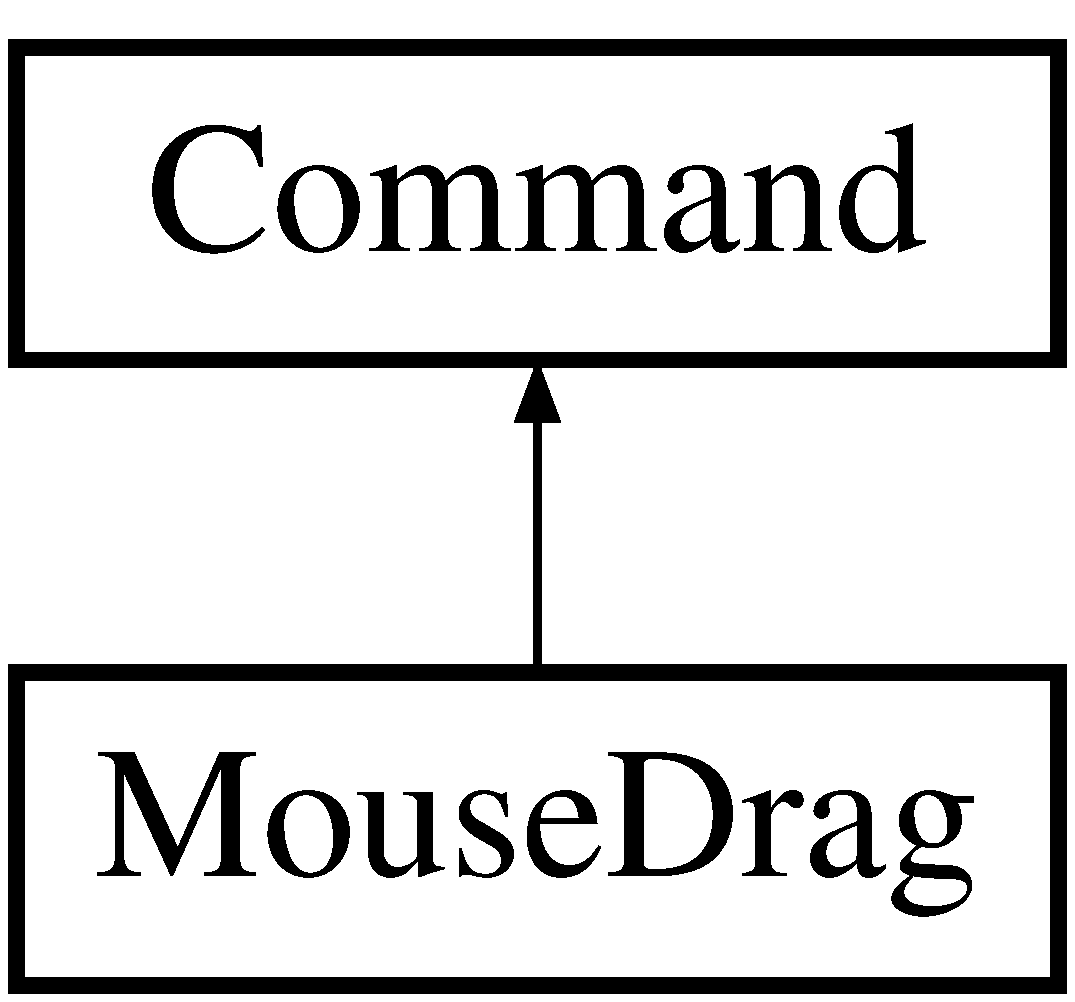
\includegraphics[height=2.000000cm]{classMouseDrag}
\end{center}
\end{figure}
\subsection*{Public Member Functions}
\begin{DoxyCompactItemize}
\item 
\hypertarget{classMouseDrag_a0548eb683710e0d6cfc97089b9083446}{void {\bfseries execute} ()}\label{classMouseDrag_a0548eb683710e0d6cfc97089b9083446}

\item 
\hypertarget{classMouseDrag_ab5be48af508bd4056c10751bb22abdfe}{void {\bfseries setxy} (int \-\_\-x, int \-\_\-y)}\label{classMouseDrag_ab5be48af508bd4056c10751bb22abdfe}

\end{DoxyCompactItemize}
\subsection*{Additional Inherited Members}


The documentation for this class was generated from the following file\-:\begin{DoxyCompactItemize}
\item 
include/\hyperlink{Commands_8h}{Commands.\-h}\end{DoxyCompactItemize}

\hypertarget{classMouseDragEnd}{\section{Mouse\-Drag\-End Class Reference}
\label{classMouseDragEnd}\index{Mouse\-Drag\-End@{Mouse\-Drag\-End}}
}
Inheritance diagram for Mouse\-Drag\-End\-:\begin{figure}[H]
\begin{center}
\leavevmode
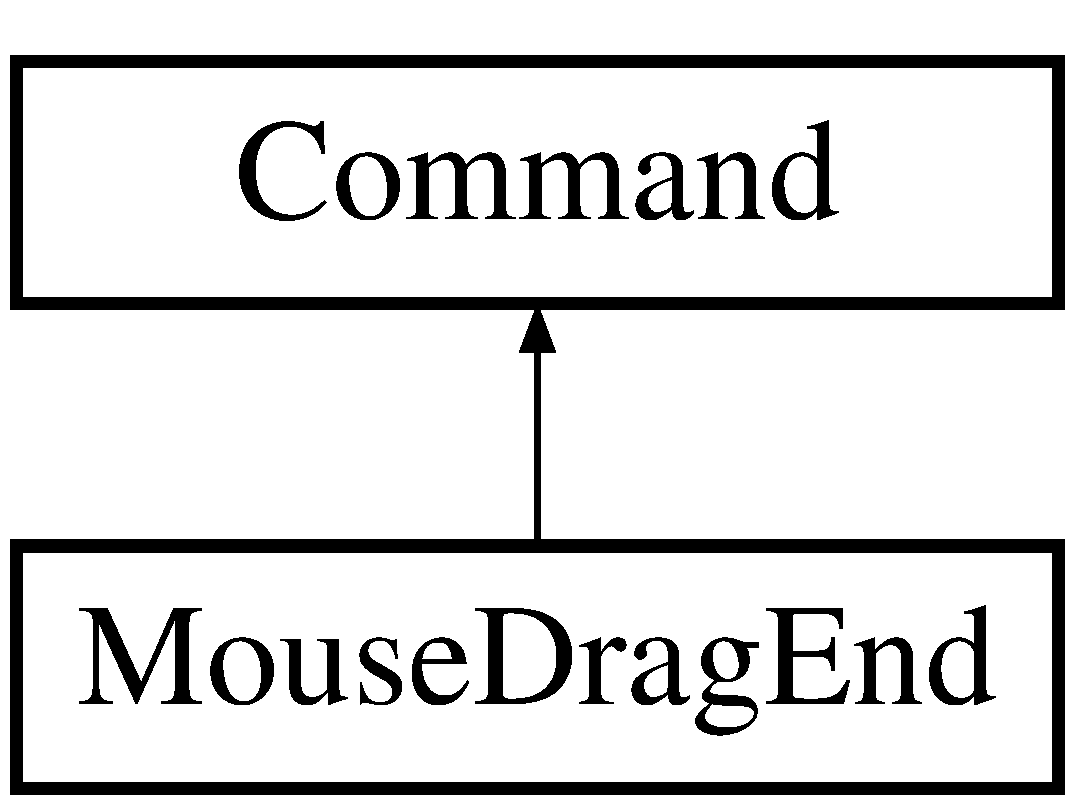
\includegraphics[height=2.000000cm]{classMouseDragEnd}
\end{center}
\end{figure}
\subsection*{Public Member Functions}
\begin{DoxyCompactItemize}
\item 
\hypertarget{classMouseDragEnd_a63fcd73eca3e643f97d9e35dc0b1238f}{void {\bfseries execute} ()}\label{classMouseDragEnd_a63fcd73eca3e643f97d9e35dc0b1238f}

\item 
\hypertarget{classMouseDragEnd_a8ae2473a78adb5ad4cf85704d5221d6c}{void {\bfseries setxy} (int \-\_\-x, int \-\_\-y)}\label{classMouseDragEnd_a8ae2473a78adb5ad4cf85704d5221d6c}

\end{DoxyCompactItemize}
\subsection*{Additional Inherited Members}


The documentation for this class was generated from the following file\-:\begin{DoxyCompactItemize}
\item 
include/\hyperlink{Commands_8h}{Commands.\-h}\end{DoxyCompactItemize}

\hypertarget{classMouseDraw}{\section{Mouse\-Draw Class Reference}
\label{classMouseDraw}\index{Mouse\-Draw@{Mouse\-Draw}}
}
Inheritance diagram for Mouse\-Draw\-:\begin{figure}[H]
\begin{center}
\leavevmode
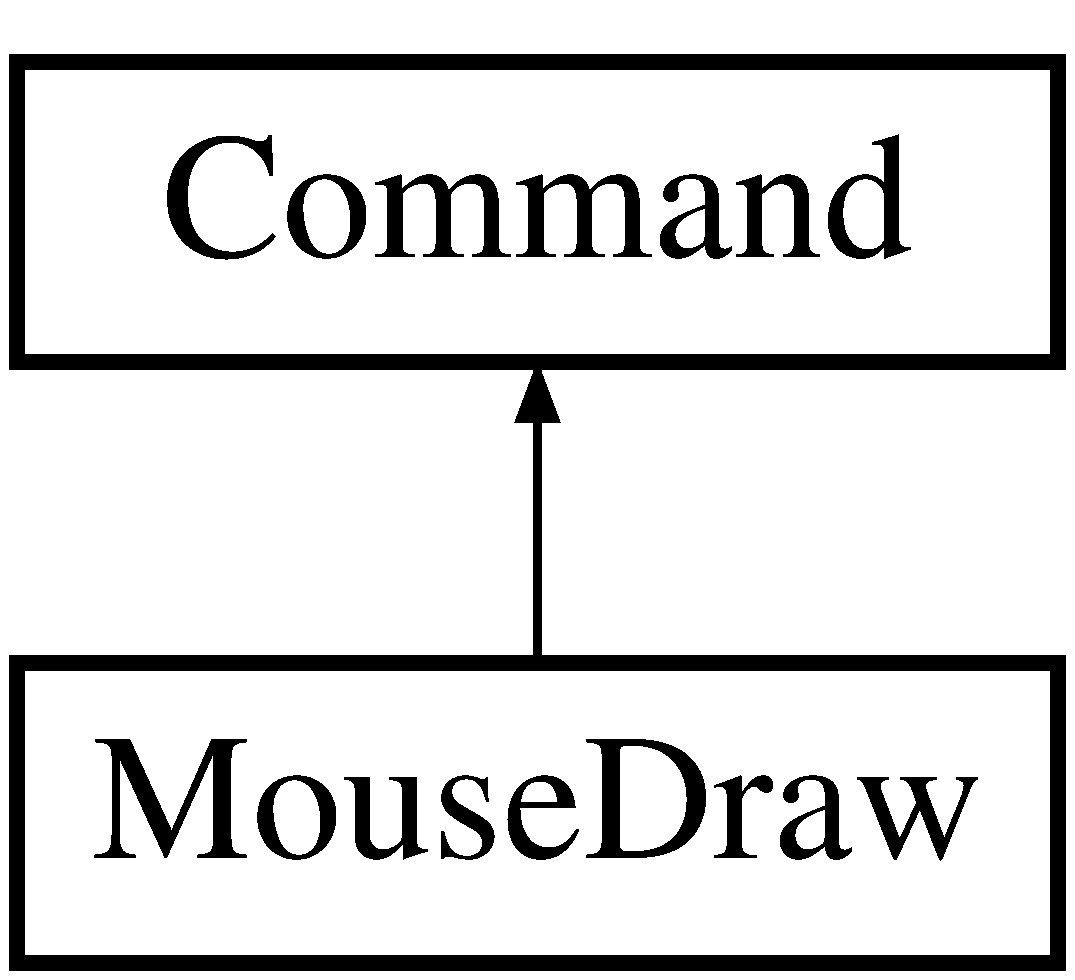
\includegraphics[height=2.000000cm]{classMouseDraw}
\end{center}
\end{figure}
\subsection*{Public Member Functions}
\begin{DoxyCompactItemize}
\item 
\hypertarget{classMouseDraw_ab0f1961e3461c2b42fd4f86e08c2737d}{void {\bfseries execute} ()}\label{classMouseDraw_ab0f1961e3461c2b42fd4f86e08c2737d}

\item 
\hypertarget{classMouseDraw_a2f43c42883ca9e8e623745bef1d03bfa}{void {\bfseries setxy} (int \-\_\-x, int \-\_\-y)}\label{classMouseDraw_a2f43c42883ca9e8e623745bef1d03bfa}

\end{DoxyCompactItemize}
\subsection*{Additional Inherited Members}


The documentation for this class was generated from the following file\-:\begin{DoxyCompactItemize}
\item 
include/\hyperlink{Commands_8h}{Commands.\-h}\end{DoxyCompactItemize}

\hypertarget{classMouseErase}{\section{Mouse\-Erase Class Reference}
\label{classMouseErase}\index{Mouse\-Erase@{Mouse\-Erase}}
}
Inheritance diagram for Mouse\-Erase\-:\begin{figure}[H]
\begin{center}
\leavevmode
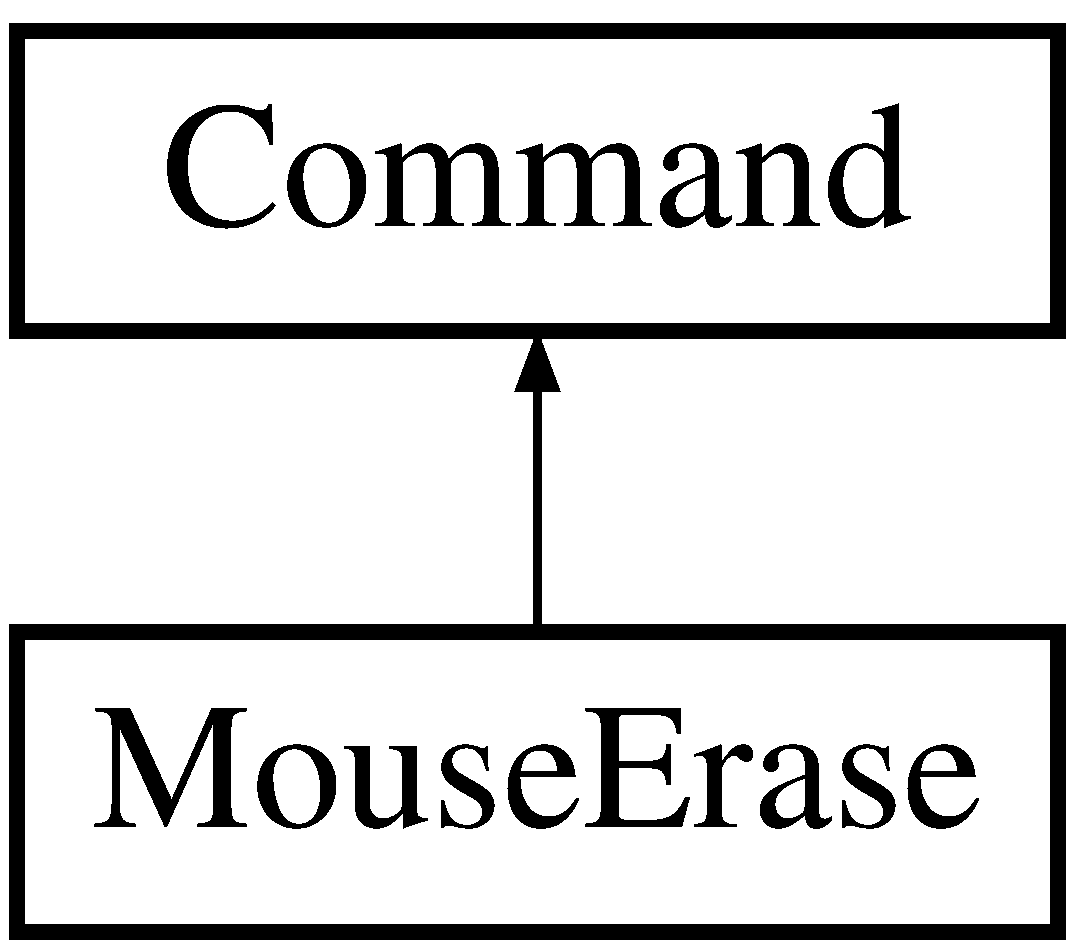
\includegraphics[height=2.000000cm]{classMouseErase}
\end{center}
\end{figure}
\subsection*{Public Member Functions}
\begin{DoxyCompactItemize}
\item 
\hypertarget{classMouseErase_aef419827cbeabf7fa59f1c73bff8b547}{void {\bfseries execute} ()}\label{classMouseErase_aef419827cbeabf7fa59f1c73bff8b547}

\item 
\hypertarget{classMouseErase_af98ce0f385ea242531537ab43a17f1ce}{void {\bfseries setxy} (int \-\_\-x, int \-\_\-y)}\label{classMouseErase_af98ce0f385ea242531537ab43a17f1ce}

\end{DoxyCompactItemize}
\subsection*{Additional Inherited Members}


The documentation for this class was generated from the following file\-:\begin{DoxyCompactItemize}
\item 
include/\hyperlink{Commands_8h}{Commands.\-h}\end{DoxyCompactItemize}

\hypertarget{classParticle}{\section{Particle Class Reference}
\label{classParticle}\index{Particle@{Particle}}
}
\subsection*{Classes}
\begin{DoxyCompactItemize}
\item 
struct \hyperlink{structParticle_1_1spring}{spring}
\end{DoxyCompactItemize}
\subsection*{Public Types}
\begin{DoxyCompactItemize}
\item 
\hypertarget{classParticle_a342eb4023785fdd39529f8ca5b994bff}{typedef struct \hyperlink{structParticle_1_1spring}{Particle\-::spring} {\bfseries Spring}}\label{classParticle_a342eb4023785fdd39529f8ca5b994bff}

\end{DoxyCompactItemize}
\subsection*{Public Member Functions}
\begin{DoxyCompactItemize}
\item 
\hypertarget{classParticle_aed0e1cc39738cf096db2b4d5f9876ac4}{{\bfseries Particle} (const \hyperlink{classParticle}{Particle} \&\-\_\-p)=default}\label{classParticle_aed0e1cc39738cf096db2b4d5f9876ac4}

\item 
\hypertarget{classParticle_a26524259b848fff0b502f6b921eef46d}{{\bfseries Particle} (\hyperlink{classVec3}{Vec3} pos=\hyperlink{classVec3}{Vec3}(), \hyperlink{classParticleProperties}{Particle\-Properties} $\ast$\-\_\-properties=N\-U\-L\-L)}\label{classParticle_a26524259b848fff0b502f6b921eef46d}

\item 
void \hyperlink{classParticle_a229585bba32aeaa9d17f66312379c015}{draw\-Particle} (const float \-\_\-pointsize)
\begin{DoxyCompactList}\small\item\em draw\-Particle draws the particle with glu\-Sphere \end{DoxyCompactList}\item 
void \hyperlink{classParticle_a308e091286c7c498080aa290243bf70d}{set\-Position} (const \hyperlink{classVec3}{Vec3} \-\_\-pos)
\begin{DoxyCompactList}\small\item\em set\-Position sets the \hyperlink{classVec3}{Vec3} position of the particle \end{DoxyCompactList}\item 
\hyperlink{classVec3}{Vec3} \hyperlink{classParticle_a471c13f167fe56ac9b5fbea5b66c07d1}{get\-Position} () const 
\begin{DoxyCompactList}\small\item\em get\-Position returns the value of the \hyperlink{classVec3}{Vec3} position of the particle \end{DoxyCompactList}\item 
void \hyperlink{classParticle_add0cb538c87ab21ba3345595adaf810e}{add\-Position} (const \hyperlink{classVec3}{Vec3} \-\_\-pos, const float \-\_\-halfheight, const float \-\_\-halfwidth, bool is3\-D)
\begin{DoxyCompactList}\small\item\em add\-Position adds a \hyperlink{classVec3}{Vec3} to current position \end{DoxyCompactList}\item 
\hypertarget{classParticle_a6b0a3046a4ab31cf0f02f883eb57acec}{void \hyperlink{classParticle_a6b0a3046a4ab31cf0f02f883eb57acec}{update\-Prev\-Position} ()}\label{classParticle_a6b0a3046a4ab31cf0f02f883eb57acec}

\begin{DoxyCompactList}\small\item\em update\-Prev\-Position updates the previous position of the particle to current position \end{DoxyCompactList}\item 
\hyperlink{classVec3}{Vec3} \hyperlink{classParticle_aebf5efcc9e99de91af2d728180017d48}{get\-Prev\-Position} () const 
\begin{DoxyCompactList}\small\item\em get\-Prev\-Position returns the previous position of the particle. Is needed to calculate particle's velocity. \end{DoxyCompactList}\item 
void \hyperlink{classParticle_ab91e3c3df102e08aa0394b2c7bd2df0e}{set\-Velocity} (const \hyperlink{classVec3}{Vec3} \-\_\-newvel)
\begin{DoxyCompactList}\small\item\em set\-Velocity sets the \hyperlink{classVec3}{Vec3} velocity of the particle \end{DoxyCompactList}\item 
\hyperlink{classVec3}{Vec3} \hyperlink{classParticle_a0fe52fbebe971ff5c4219f0ecf3b8941}{get\-Velocity} () const 
\begin{DoxyCompactList}\small\item\em get\-Velocity returns the current velocity of the particle \end{DoxyCompactList}\item 
void \hyperlink{classParticle_af86bd61b41085f3bb390bb6ddc0734d7}{add\-Velocity} (const \hyperlink{classVec3}{Vec3} addedvel)
\begin{DoxyCompactList}\small\item\em add\-Velocity adds a \hyperlink{classVec3}{Vec3} to current velocity of particle \end{DoxyCompactList}\item 
void \hyperlink{classParticle_ad316202f5c32510b970c2142c6ca65d1}{update\-Position} (double elapsedtime, float halfheight, float halfwidth, bool is3\-D)
\begin{DoxyCompactList}\small\item\em update\-Position updates the position according to particle's velocity \end{DoxyCompactList}\item 
int \hyperlink{classParticle_afcae0c2dba5f4158384448b9004ee88a}{get\-Grid\-Position} () const 
\begin{DoxyCompactList}\small\item\em get\-Grid\-Position returns the spatial hash grid index \end{DoxyCompactList}\item 
void \hyperlink{classParticle_a4cb304dc5863a08d7f3d1c456bccb598}{set\-Grid\-Position} (int p)
\begin{DoxyCompactList}\small\item\em set\-Grid\-Position sets the value inside the particle representing the spatial hash grid index \end{DoxyCompactList}\item 
void \hyperlink{classParticle_aa715f6f18f8257fb31a7755c18cfda22}{set\-Drag} (bool drag)
\begin{DoxyCompactList}\small\item\em set\-Drag sets the drag bool which shows whether the particle is being dragged by the mouse or not \end{DoxyCompactList}\item 
bool \hyperlink{classParticle_a57c96039de3e090bfd9fc3fcc5923ab0}{get\-Drag} () const 
\begin{DoxyCompactList}\small\item\em get\-Drag sets the drag bool which shows whether the particle is being dragged by the mouse or not \end{DoxyCompactList}\item 
bool \hyperlink{classParticle_af8a2db33e42e0e4ed3da7dfe04e67b05}{get\-Wall} () const 
\begin{DoxyCompactList}\small\item\em get\-Wall returns the bool that shows whether the particle is static or not \end{DoxyCompactList}\item 
void \hyperlink{classParticle_a930c48cf6e8fe1212409f92c68774e0f}{set\-Wall} (bool newwall)
\begin{DoxyCompactList}\small\item\em set\-Wall returns the bool that shows whether the particle is static or not \end{DoxyCompactList}\item 
\hypertarget{classParticle_a96d696c7db5c7f96ee2d5d9fae5cee52}{void \hyperlink{classParticle_a96d696c7db5c7f96ee2d5d9fae5cee52}{set\-Is\-Object} ()}\label{classParticle_a96d696c7db5c7f96ee2d5d9fae5cee52}

\begin{DoxyCompactList}\small\item\em set\-Is\-Object sets the object bool on the particle. This means it keeps it's springs and makes no new one. \end{DoxyCompactList}\item 
bool \hyperlink{classParticle_aa4b116b621e88c3dd422520d6631e6d9}{is\-Object} ()
\begin{DoxyCompactList}\small\item\em is\-Object returns the object bool on the particle. \end{DoxyCompactList}\item 
\hypertarget{classParticle_a65da6bc58018b897087371b3db4606e9}{void \hyperlink{classParticle_a65da6bc58018b897087371b3db4606e9}{set\-Init} ()}\label{classParticle_a65da6bc58018b897087371b3db4606e9}

\begin{DoxyCompactList}\small\item\em set\-Init m\-\_\-init is set when the particle's springs have been made. Is used only when particle is part of an object (m\-\_\-is\-Part\-Of\-Object==true); \end{DoxyCompactList}\item 
bool \hyperlink{classParticle_ae1b9331af6c436952ebe3a748703355b}{is\-Init} ()
\begin{DoxyCompactList}\small\item\em is\-Init returns the value of m\-\_\-init \end{DoxyCompactList}\item 
void \hyperlink{classParticle_ae84d5233185dda1df8d92b31988c5790}{set\-Alive} (bool \-\_\-i)
\begin{DoxyCompactList}\small\item\em set\-Alive sets m\-\_\-alive to new bool. \end{DoxyCompactList}\item 
bool \hyperlink{classParticle_aca953a26773ae228530de02c2becf6d7}{get\-Alive} ()
\begin{DoxyCompactList}\small\item\em get\-Alive returns value of m\-\_\-alive \end{DoxyCompactList}\item 
void \hyperlink{classParticle_a984ce8220a48ee851bfaa443cc98ae96}{set\-Index} (int \-\_\-i)
\begin{DoxyCompactList}\small\item\em set\-Index sets m\-\_\-index which is index of particle inside world's vector m\-\_\-particles \end{DoxyCompactList}\item 
int \hyperlink{classParticle_a0cb31e8c8a445894f2f5b68b148135d2}{get\-Index} ()
\begin{DoxyCompactList}\small\item\em get\-Index returns m\-\_\-index which is index of particle inside world's vector m\-\_\-particles \end{DoxyCompactList}\item 
void \hyperlink{classParticle_ae82fd88a76aa1c0aaa6c6d2149401ed2}{update\-Spring\-Index} (int \-\_\-from, int \-\_\-to)
\begin{DoxyCompactList}\small\item\em update\-Spring\-Index checks if there is a spring with index from and if so changes it to to if to == -\/1 then it deletes that spring index from particle\-Springs \end{DoxyCompactList}\item 
\hyperlink{classParticleProperties}{Particle\-Properties} $\ast$ \hyperlink{classParticle_aa8d3d0b59174d90b174497a2b0eecf53}{get\-Properties} () const 
\begin{DoxyCompactList}\small\item\em get\-Properties returns pointer to the \hyperlink{classParticleProperties}{Particle\-Properties} object the particle has \end{DoxyCompactList}\end{DoxyCompactItemize}
\subsection*{Public Attributes}
\begin{DoxyCompactItemize}
\item 
\hypertarget{classParticle_a915dc46195fba62472c8322976fb4c3f}{std\-::vector$<$ int $>$ \hyperlink{classParticle_a915dc46195fba62472c8322976fb4c3f}{m\-\_\-particle\-Springs}}\label{classParticle_a915dc46195fba62472c8322976fb4c3f}

\begin{DoxyCompactList}\small\item\em particle\-Springs vector of spring indexes that the particle is attached to. It is public as we need to loop through these inside of world. \end{DoxyCompactList}\end{DoxyCompactItemize}


\subsection{Member Function Documentation}
\hypertarget{classParticle_add0cb538c87ab21ba3345595adaf810e}{\index{Particle@{Particle}!add\-Position@{add\-Position}}
\index{add\-Position@{add\-Position}!Particle@{Particle}}
\subsubsection[{add\-Position}]{\setlength{\rightskip}{0pt plus 5cm}void Particle\-::add\-Position (
\begin{DoxyParamCaption}
\item[{const {\bf Vec3}}]{\-\_\-pos, }
\item[{const float}]{\-\_\-halfheight, }
\item[{const float}]{\-\_\-halfwidth, }
\item[{bool}]{is3\-D}
\end{DoxyParamCaption}
)}}\label{classParticle_add0cb538c87ab21ba3345595adaf810e}


add\-Position adds a \hyperlink{classVec3}{Vec3} to current position 


\begin{DoxyParams}[1]{Parameters}
\mbox{\tt in}  & {\em \-\_\-pos} & \hyperlink{classVec3}{Vec3} to add to particle's position \\
\hline
\mbox{\tt in}  & {\em \-\_\-halfheight} & makes sure particle does not leave the boundaries \\
\hline
\mbox{\tt in}  & {\em \-\_\-halfwidth} & makes sure particle does not leave the boundaries \\
\hline
\end{DoxyParams}
\hypertarget{classParticle_af86bd61b41085f3bb390bb6ddc0734d7}{\index{Particle@{Particle}!add\-Velocity@{add\-Velocity}}
\index{add\-Velocity@{add\-Velocity}!Particle@{Particle}}
\subsubsection[{add\-Velocity}]{\setlength{\rightskip}{0pt plus 5cm}void Particle\-::add\-Velocity (
\begin{DoxyParamCaption}
\item[{const {\bf Vec3}}]{addedvel}
\end{DoxyParamCaption}
)}}\label{classParticle_af86bd61b41085f3bb390bb6ddc0734d7}


add\-Velocity adds a \hyperlink{classVec3}{Vec3} to current velocity of particle 


\begin{DoxyParams}[1]{Parameters}
\mbox{\tt in}  & {\em \-\_\-addedvel} & \hyperlink{classVec3}{Vec3} to add to particle's velocity \\
\hline
\end{DoxyParams}
\hypertarget{classParticle_a229585bba32aeaa9d17f66312379c015}{\index{Particle@{Particle}!draw\-Particle@{draw\-Particle}}
\index{draw\-Particle@{draw\-Particle}!Particle@{Particle}}
\subsubsection[{draw\-Particle}]{\setlength{\rightskip}{0pt plus 5cm}void Particle\-::draw\-Particle (
\begin{DoxyParamCaption}
\item[{const float}]{\-\_\-pointsize}
\end{DoxyParamCaption}
)}}\label{classParticle_a229585bba32aeaa9d17f66312379c015}


draw\-Particle draws the particle with glu\-Sphere 


\begin{DoxyParams}[1]{Parameters}
\mbox{\tt in}  & {\em \-\_\-pointsize} & size of sphere \\
\hline
\end{DoxyParams}
\hypertarget{classParticle_aca953a26773ae228530de02c2becf6d7}{\index{Particle@{Particle}!get\-Alive@{get\-Alive}}
\index{get\-Alive@{get\-Alive}!Particle@{Particle}}
\subsubsection[{get\-Alive}]{\setlength{\rightskip}{0pt plus 5cm}bool Particle\-::get\-Alive (
\begin{DoxyParamCaption}
{}
\end{DoxyParamCaption}
)}}\label{classParticle_aca953a26773ae228530de02c2becf6d7}


get\-Alive returns value of m\-\_\-alive 

\begin{DoxyReturn}{Returns}
m\-\_\-alive value 
\end{DoxyReturn}
\hypertarget{classParticle_a57c96039de3e090bfd9fc3fcc5923ab0}{\index{Particle@{Particle}!get\-Drag@{get\-Drag}}
\index{get\-Drag@{get\-Drag}!Particle@{Particle}}
\subsubsection[{get\-Drag}]{\setlength{\rightskip}{0pt plus 5cm}bool Particle\-::get\-Drag (
\begin{DoxyParamCaption}
{}
\end{DoxyParamCaption}
) const}}\label{classParticle_a57c96039de3e090bfd9fc3fcc5923ab0}


get\-Drag sets the drag bool which shows whether the particle is being dragged by the mouse or not 

\begin{DoxyReturn}{Returns}
drag bool 
\end{DoxyReturn}
\hypertarget{classParticle_afcae0c2dba5f4158384448b9004ee88a}{\index{Particle@{Particle}!get\-Grid\-Position@{get\-Grid\-Position}}
\index{get\-Grid\-Position@{get\-Grid\-Position}!Particle@{Particle}}
\subsubsection[{get\-Grid\-Position}]{\setlength{\rightskip}{0pt plus 5cm}int Particle\-::get\-Grid\-Position (
\begin{DoxyParamCaption}
{}
\end{DoxyParamCaption}
) const}}\label{classParticle_afcae0c2dba5f4158384448b9004ee88a}


get\-Grid\-Position returns the spatial hash grid index 

\begin{DoxyReturn}{Returns}
spatial hash index for particle 
\end{DoxyReturn}
\hypertarget{classParticle_a0cb31e8c8a445894f2f5b68b148135d2}{\index{Particle@{Particle}!get\-Index@{get\-Index}}
\index{get\-Index@{get\-Index}!Particle@{Particle}}
\subsubsection[{get\-Index}]{\setlength{\rightskip}{0pt plus 5cm}int Particle\-::get\-Index (
\begin{DoxyParamCaption}
{}
\end{DoxyParamCaption}
)}}\label{classParticle_a0cb31e8c8a445894f2f5b68b148135d2}


get\-Index returns m\-\_\-index which is index of particle inside world's vector m\-\_\-particles 

\begin{DoxyReturn}{Returns}
bool value of m\-\_\-index 
\end{DoxyReturn}
\hypertarget{classParticle_a471c13f167fe56ac9b5fbea5b66c07d1}{\index{Particle@{Particle}!get\-Position@{get\-Position}}
\index{get\-Position@{get\-Position}!Particle@{Particle}}
\subsubsection[{get\-Position}]{\setlength{\rightskip}{0pt plus 5cm}{\bf Vec3} Particle\-::get\-Position (
\begin{DoxyParamCaption}
{}
\end{DoxyParamCaption}
) const}}\label{classParticle_a471c13f167fe56ac9b5fbea5b66c07d1}


get\-Position returns the value of the \hyperlink{classVec3}{Vec3} position of the particle 

\begin{DoxyReturn}{Returns}
\hyperlink{classVec3}{Vec3} position of particle 
\end{DoxyReturn}
\hypertarget{classParticle_aebf5efcc9e99de91af2d728180017d48}{\index{Particle@{Particle}!get\-Prev\-Position@{get\-Prev\-Position}}
\index{get\-Prev\-Position@{get\-Prev\-Position}!Particle@{Particle}}
\subsubsection[{get\-Prev\-Position}]{\setlength{\rightskip}{0pt plus 5cm}{\bf Vec3} Particle\-::get\-Prev\-Position (
\begin{DoxyParamCaption}
{}
\end{DoxyParamCaption}
) const}}\label{classParticle_aebf5efcc9e99de91af2d728180017d48}


get\-Prev\-Position returns the previous position of the particle. Is needed to calculate particle's velocity. 

\begin{DoxyReturn}{Returns}
\hyperlink{classVec3}{Vec3} of previous position 
\end{DoxyReturn}
\hypertarget{classParticle_aa8d3d0b59174d90b174497a2b0eecf53}{\index{Particle@{Particle}!get\-Properties@{get\-Properties}}
\index{get\-Properties@{get\-Properties}!Particle@{Particle}}
\subsubsection[{get\-Properties}]{\setlength{\rightskip}{0pt plus 5cm}{\bf Particle\-Properties}$\ast$ Particle\-::get\-Properties (
\begin{DoxyParamCaption}
{}
\end{DoxyParamCaption}
) const}}\label{classParticle_aa8d3d0b59174d90b174497a2b0eecf53}


get\-Properties returns pointer to the \hyperlink{classParticleProperties}{Particle\-Properties} object the particle has 

\begin{DoxyReturn}{Returns}
$\ast$\-Particle\-Properties of the particle 
\end{DoxyReturn}
\hypertarget{classParticle_a0fe52fbebe971ff5c4219f0ecf3b8941}{\index{Particle@{Particle}!get\-Velocity@{get\-Velocity}}
\index{get\-Velocity@{get\-Velocity}!Particle@{Particle}}
\subsubsection[{get\-Velocity}]{\setlength{\rightskip}{0pt plus 5cm}{\bf Vec3} Particle\-::get\-Velocity (
\begin{DoxyParamCaption}
{}
\end{DoxyParamCaption}
) const}}\label{classParticle_a0fe52fbebe971ff5c4219f0ecf3b8941}


get\-Velocity returns the current velocity of the particle 

\begin{DoxyReturn}{Returns}
\hyperlink{classVec3}{Vec3} velocity of particle 
\end{DoxyReturn}
\hypertarget{classParticle_af8a2db33e42e0e4ed3da7dfe04e67b05}{\index{Particle@{Particle}!get\-Wall@{get\-Wall}}
\index{get\-Wall@{get\-Wall}!Particle@{Particle}}
\subsubsection[{get\-Wall}]{\setlength{\rightskip}{0pt plus 5cm}bool Particle\-::get\-Wall (
\begin{DoxyParamCaption}
{}
\end{DoxyParamCaption}
) const}}\label{classParticle_af8a2db33e42e0e4ed3da7dfe04e67b05}


get\-Wall returns the bool that shows whether the particle is static or not 

\begin{DoxyReturn}{Returns}
the wall bool 
\end{DoxyReturn}
\hypertarget{classParticle_ae1b9331af6c436952ebe3a748703355b}{\index{Particle@{Particle}!is\-Init@{is\-Init}}
\index{is\-Init@{is\-Init}!Particle@{Particle}}
\subsubsection[{is\-Init}]{\setlength{\rightskip}{0pt plus 5cm}bool Particle\-::is\-Init (
\begin{DoxyParamCaption}
{}
\end{DoxyParamCaption}
)}}\label{classParticle_ae1b9331af6c436952ebe3a748703355b}


is\-Init returns the value of m\-\_\-init 

\begin{DoxyReturn}{Returns}
m\-\_\-init bool value 
\end{DoxyReturn}
\hypertarget{classParticle_aa4b116b621e88c3dd422520d6631e6d9}{\index{Particle@{Particle}!is\-Object@{is\-Object}}
\index{is\-Object@{is\-Object}!Particle@{Particle}}
\subsubsection[{is\-Object}]{\setlength{\rightskip}{0pt plus 5cm}bool Particle\-::is\-Object (
\begin{DoxyParamCaption}
{}
\end{DoxyParamCaption}
)}}\label{classParticle_aa4b116b621e88c3dd422520d6631e6d9}


is\-Object returns the object bool on the particle. 

\begin{DoxyReturn}{Returns}
bool that shows whether particle is an object 
\end{DoxyReturn}
\hypertarget{classParticle_ae84d5233185dda1df8d92b31988c5790}{\index{Particle@{Particle}!set\-Alive@{set\-Alive}}
\index{set\-Alive@{set\-Alive}!Particle@{Particle}}
\subsubsection[{set\-Alive}]{\setlength{\rightskip}{0pt plus 5cm}void Particle\-::set\-Alive (
\begin{DoxyParamCaption}
\item[{bool}]{\-\_\-i}
\end{DoxyParamCaption}
)}}\label{classParticle_ae84d5233185dda1df8d92b31988c5790}


set\-Alive sets m\-\_\-alive to new bool. 


\begin{DoxyParams}[1]{Parameters}
\mbox{\tt in}  & {\em \-\_\-i} & bool to set m\-\_\-alive to \\
\hline
\end{DoxyParams}
\hypertarget{classParticle_aa715f6f18f8257fb31a7755c18cfda22}{\index{Particle@{Particle}!set\-Drag@{set\-Drag}}
\index{set\-Drag@{set\-Drag}!Particle@{Particle}}
\subsubsection[{set\-Drag}]{\setlength{\rightskip}{0pt plus 5cm}void Particle\-::set\-Drag (
\begin{DoxyParamCaption}
\item[{bool}]{drag}
\end{DoxyParamCaption}
)}}\label{classParticle_aa715f6f18f8257fb31a7755c18cfda22}


set\-Drag sets the drag bool which shows whether the particle is being dragged by the mouse or not 


\begin{DoxyParams}[1]{Parameters}
\mbox{\tt in}  & {\em \-\_\-drag} & the bool to set m\-\_\-drag to \\
\hline
\end{DoxyParams}
\hypertarget{classParticle_a4cb304dc5863a08d7f3d1c456bccb598}{\index{Particle@{Particle}!set\-Grid\-Position@{set\-Grid\-Position}}
\index{set\-Grid\-Position@{set\-Grid\-Position}!Particle@{Particle}}
\subsubsection[{set\-Grid\-Position}]{\setlength{\rightskip}{0pt plus 5cm}void Particle\-::set\-Grid\-Position (
\begin{DoxyParamCaption}
\item[{int}]{p}
\end{DoxyParamCaption}
)}}\label{classParticle_a4cb304dc5863a08d7f3d1c456bccb598}


set\-Grid\-Position sets the value inside the particle representing the spatial hash grid index 


\begin{DoxyParams}[1]{Parameters}
\mbox{\tt in}  & {\em \-\_\-p} & int to set the index to \\
\hline
\end{DoxyParams}
\hypertarget{classParticle_a984ce8220a48ee851bfaa443cc98ae96}{\index{Particle@{Particle}!set\-Index@{set\-Index}}
\index{set\-Index@{set\-Index}!Particle@{Particle}}
\subsubsection[{set\-Index}]{\setlength{\rightskip}{0pt plus 5cm}void Particle\-::set\-Index (
\begin{DoxyParamCaption}
\item[{int}]{\-\_\-i}
\end{DoxyParamCaption}
)}}\label{classParticle_a984ce8220a48ee851bfaa443cc98ae96}


set\-Index sets m\-\_\-index which is index of particle inside world's vector m\-\_\-particles 


\begin{DoxyParams}[1]{Parameters}
\mbox{\tt in}  & {\em \-\_\-i} & new value of m\-\_\-index to be set \\
\hline
\end{DoxyParams}
\hypertarget{classParticle_a308e091286c7c498080aa290243bf70d}{\index{Particle@{Particle}!set\-Position@{set\-Position}}
\index{set\-Position@{set\-Position}!Particle@{Particle}}
\subsubsection[{set\-Position}]{\setlength{\rightskip}{0pt plus 5cm}void Particle\-::set\-Position (
\begin{DoxyParamCaption}
\item[{const {\bf Vec3}}]{\-\_\-pos}
\end{DoxyParamCaption}
)}}\label{classParticle_a308e091286c7c498080aa290243bf70d}


set\-Position sets the \hyperlink{classVec3}{Vec3} position of the particle 


\begin{DoxyParams}[1]{Parameters}
\mbox{\tt in}  & {\em pos} & position to be set to \\
\hline
\end{DoxyParams}
\hypertarget{classParticle_ab91e3c3df102e08aa0394b2c7bd2df0e}{\index{Particle@{Particle}!set\-Velocity@{set\-Velocity}}
\index{set\-Velocity@{set\-Velocity}!Particle@{Particle}}
\subsubsection[{set\-Velocity}]{\setlength{\rightskip}{0pt plus 5cm}void Particle\-::set\-Velocity (
\begin{DoxyParamCaption}
\item[{const {\bf Vec3}}]{\-\_\-newvel}
\end{DoxyParamCaption}
)}}\label{classParticle_ab91e3c3df102e08aa0394b2c7bd2df0e}


set\-Velocity sets the \hyperlink{classVec3}{Vec3} velocity of the particle 


\begin{DoxyParams}[1]{Parameters}
\mbox{\tt in}  & {\em \-\_\-newvel} & \hyperlink{classVec3}{Vec3} velocity to set particle's velocity \\
\hline
\end{DoxyParams}
\hypertarget{classParticle_a930c48cf6e8fe1212409f92c68774e0f}{\index{Particle@{Particle}!set\-Wall@{set\-Wall}}
\index{set\-Wall@{set\-Wall}!Particle@{Particle}}
\subsubsection[{set\-Wall}]{\setlength{\rightskip}{0pt plus 5cm}void Particle\-::set\-Wall (
\begin{DoxyParamCaption}
\item[{bool}]{newwall}
\end{DoxyParamCaption}
)}}\label{classParticle_a930c48cf6e8fe1212409f92c68774e0f}


set\-Wall returns the bool that shows whether the particle is static or not 


\begin{DoxyParams}{Parameters}
{\em newwall} & the bool to set m\-\_\-wall to \\
\hline
\end{DoxyParams}
\hypertarget{classParticle_ad316202f5c32510b970c2142c6ca65d1}{\index{Particle@{Particle}!update\-Position@{update\-Position}}
\index{update\-Position@{update\-Position}!Particle@{Particle}}
\subsubsection[{update\-Position}]{\setlength{\rightskip}{0pt plus 5cm}void Particle\-::update\-Position (
\begin{DoxyParamCaption}
\item[{double}]{elapsedtime, }
\item[{float}]{halfheight, }
\item[{float}]{halfwidth, }
\item[{bool}]{is3\-D}
\end{DoxyParamCaption}
)}}\label{classParticle_ad316202f5c32510b970c2142c6ca65d1}


update\-Position updates the position according to particle's velocity 


\begin{DoxyParams}[1]{Parameters}
\mbox{\tt in}  & {\em \-\_\-elapsedtime} & multiplies the velocity according to this timestep \\
\hline
\mbox{\tt in}  & {\em \-\_\-halfheight} & makes sure particle does not leave the boundaries \\
\hline
\mbox{\tt in}  & {\em \-\_\-halfwidth} & makes sure particle does not leave the boundaries \\
\hline
\end{DoxyParams}
\hypertarget{classParticle_ae82fd88a76aa1c0aaa6c6d2149401ed2}{\index{Particle@{Particle}!update\-Spring\-Index@{update\-Spring\-Index}}
\index{update\-Spring\-Index@{update\-Spring\-Index}!Particle@{Particle}}
\subsubsection[{update\-Spring\-Index}]{\setlength{\rightskip}{0pt plus 5cm}void Particle\-::update\-Spring\-Index (
\begin{DoxyParamCaption}
\item[{int}]{\-\_\-from, }
\item[{int}]{\-\_\-to}
\end{DoxyParamCaption}
)}}\label{classParticle_ae82fd88a76aa1c0aaa6c6d2149401ed2}


update\-Spring\-Index checks if there is a spring with index from and if so changes it to to if to == -\/1 then it deletes that spring index from particle\-Springs 


\begin{DoxyParams}[1]{Parameters}
\mbox{\tt in}  & {\em \-\_\-from} & index of spring to change \\
\hline
\mbox{\tt in}  & {\em \-\_\-to} & index of spring to change to \\
\hline
\end{DoxyParams}


The documentation for this class was generated from the following file\-:\begin{DoxyCompactItemize}
\item 
include/\hyperlink{Particle_8h}{Particle.\-h}\end{DoxyCompactItemize}

\hypertarget{classParticleProperties}{\section{Particle\-Properties Class Reference}
\label{classParticleProperties}\index{Particle\-Properties@{Particle\-Properties}}
}
\subsection*{Public Member Functions}
\begin{DoxyCompactItemize}
\item 
\hypertarget{classParticleProperties_aa1d8a02182b9264effb3d08adbe02c4f}{{\bfseries Particle\-Properties} (bool spring=false, G\-Lfloat \-\_\-sigma=0.\-05f, G\-Lfloat \-\_\-beta=0.\-1f, G\-Lfloat \-\_\-gamma=0.\-004f, G\-Lfloat \-\_\-alpha=0.\-3f, G\-Lfloat \-\_\-knear=0.\-01f, G\-Lfloat \-\_\-k=0.\-004f, G\-Lfloat \-\_\-kspring=0.\-3f, G\-Lfloat \-\_\-p0=5.\-0f, G\-Lfloat \-\_\-red=0, G\-Lfloat \-\_\-green=0, G\-Lfloat \-\_\-blue=1.\-0f, bool \-\_\-coloureffect=true)}\label{classParticleProperties_aa1d8a02182b9264effb3d08adbe02c4f}

\item 
\hypertarget{classParticleProperties_aca9ff4ec7aea1b683873692781b7d2e7}{G\-Lfloat {\bfseries get\-Sigma} () const }\label{classParticleProperties_aca9ff4ec7aea1b683873692781b7d2e7}

\item 
\hypertarget{classParticleProperties_a9ef419fe9734102022bb7612e6caebdf}{G\-Lfloat {\bfseries get\-Beta} () const }\label{classParticleProperties_a9ef419fe9734102022bb7612e6caebdf}

\item 
\hypertarget{classParticleProperties_a072d0400633c0cf1cab12de27dbf6b61}{G\-Lfloat {\bfseries get\-Gamma} () const }\label{classParticleProperties_a072d0400633c0cf1cab12de27dbf6b61}

\item 
\hypertarget{classParticleProperties_a7cd807f48b68ec5f333f4f0a13e8f72e}{G\-Lfloat {\bfseries get\-Alpha} () const }\label{classParticleProperties_a7cd807f48b68ec5f333f4f0a13e8f72e}

\item 
\hypertarget{classParticleProperties_af389c50eb3f1a32f25d121888a65276f}{G\-Lfloat {\bfseries get\-Knear} () const }\label{classParticleProperties_af389c50eb3f1a32f25d121888a65276f}

\item 
\hypertarget{classParticleProperties_a06234cb1c152001040a06e5f551656a1}{G\-Lfloat {\bfseries get\-K} () const }\label{classParticleProperties_a06234cb1c152001040a06e5f551656a1}

\item 
\hypertarget{classParticleProperties_a31a3825b69b29db36087eddcfcee315e}{G\-Lfloat {\bfseries get\-Kspring} () const }\label{classParticleProperties_a31a3825b69b29db36087eddcfcee315e}

\item 
\hypertarget{classParticleProperties_a53b2dfc0c3c78a0104a1791d0b977c8b}{G\-Lfloat {\bfseries get\-Red} () const }\label{classParticleProperties_a53b2dfc0c3c78a0104a1791d0b977c8b}

\item 
\hypertarget{classParticleProperties_a6f50c8d89a1d66940375261b239bb8a6}{G\-Lfloat {\bfseries get\-Green} () const }\label{classParticleProperties_a6f50c8d89a1d66940375261b239bb8a6}

\item 
\hypertarget{classParticleProperties_a9f44172411197d3bf972dab70c45838d}{G\-Lfloat {\bfseries get\-Blue} () const }\label{classParticleProperties_a9f44172411197d3bf972dab70c45838d}

\item 
\hypertarget{classParticleProperties_a00fb572953359318f908c5550623de99}{G\-Lfloat {\bfseries get\-P0} () const }\label{classParticleProperties_a00fb572953359318f908c5550623de99}

\item 
\hypertarget{classParticleProperties_a77a36791ca589cc5e2e25cda1e05ae44}{bool {\bfseries get\-Spring} () const }\label{classParticleProperties_a77a36791ca589cc5e2e25cda1e05ae44}

\item 
\hypertarget{classParticleProperties_a9fef64994d9b7d77bd3b2da3ac2fa9ae}{bool {\bfseries get\-Colour\-Effect} () const }\label{classParticleProperties_a9fef64994d9b7d77bd3b2da3ac2fa9ae}

\item 
\hypertarget{classParticleProperties_a4a9760c2c8b48ed4b83c9561a34a594d}{void \hyperlink{classParticleProperties_a4a9760c2c8b48ed4b83c9561a34a594d}{print\-Variables} () const }\label{classParticleProperties_a4a9760c2c8b48ed4b83c9561a34a594d}

\begin{DoxyCompactList}\small\item\em print\-Variables prints the attributes. Used when randomizing \hyperlink{classParticleProperties}{Particle\-Properties}. \end{DoxyCompactList}\item 
void \hyperlink{classParticleProperties_ad19947a218ea62516bc5f0975fb86d87}{randomize} (int \-\_\-seed)
\begin{DoxyCompactList}\small\item\em randomize randomizes the attributes of the object \end{DoxyCompactList}\end{DoxyCompactItemize}


\subsection{Member Function Documentation}
\hypertarget{classParticleProperties_ad19947a218ea62516bc5f0975fb86d87}{\index{Particle\-Properties@{Particle\-Properties}!randomize@{randomize}}
\index{randomize@{randomize}!ParticleProperties@{Particle\-Properties}}
\subsubsection[{randomize}]{\setlength{\rightskip}{0pt plus 5cm}void Particle\-Properties\-::randomize (
\begin{DoxyParamCaption}
\item[{int}]{\-\_\-seed}
\end{DoxyParamCaption}
)}}\label{classParticleProperties_ad19947a218ea62516bc5f0975fb86d87}


randomize randomizes the attributes of the object 


\begin{DoxyParams}[1]{Parameters}
\mbox{\tt in}  & {\em \-\_\-seed} & the srand() input, same seed same, \hyperlink{classParticleProperties}{Particle\-Properties} attributes \\
\hline
\end{DoxyParams}


The documentation for this class was generated from the following file\-:\begin{DoxyCompactItemize}
\item 
include/\hyperlink{ParticleProperties_8h}{Particle\-Properties.\-h}\end{DoxyCompactItemize}

\hypertarget{classResizeWorld}{\section{Resize\-World Class Reference}
\label{classResizeWorld}\index{Resize\-World@{Resize\-World}}
}
Inheritance diagram for Resize\-World\-:\begin{figure}[H]
\begin{center}
\leavevmode
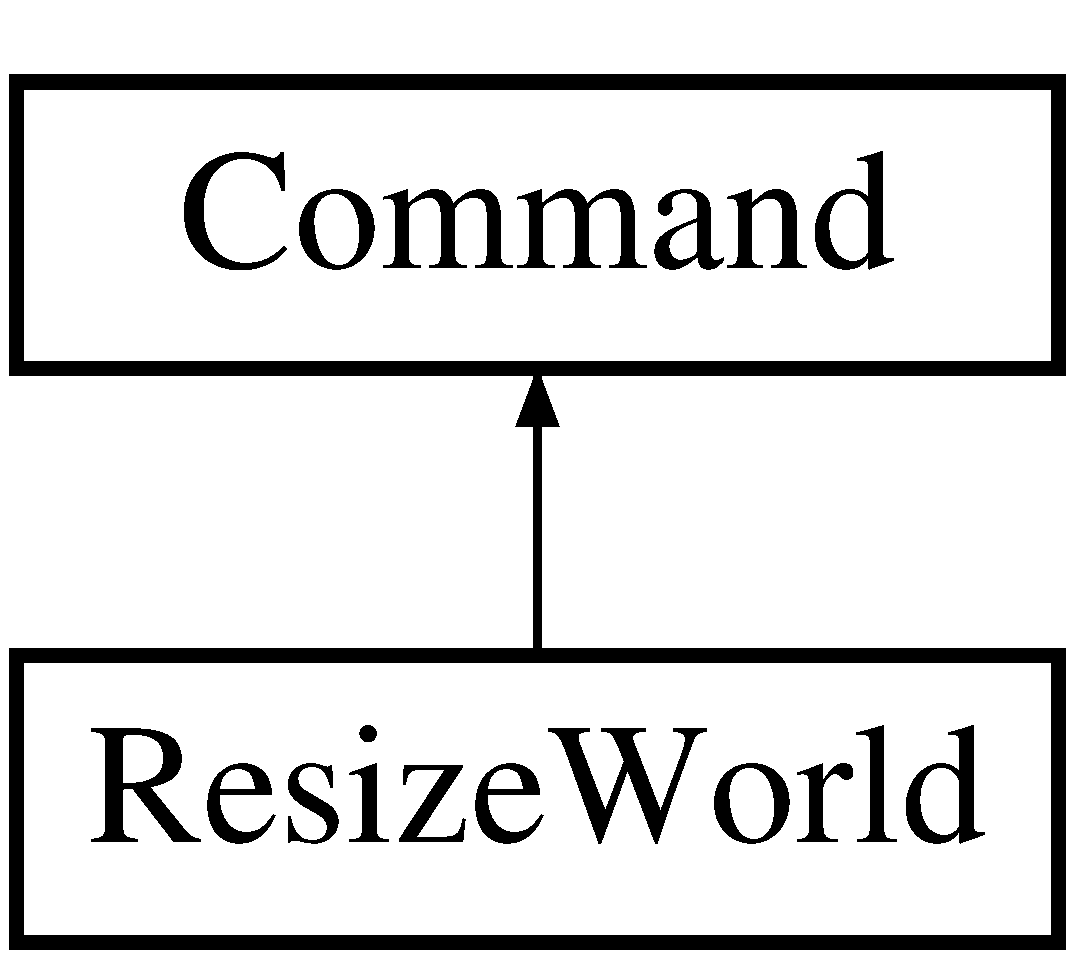
\includegraphics[height=2.000000cm]{classResizeWorld}
\end{center}
\end{figure}
\subsection*{Public Member Functions}
\begin{DoxyCompactItemize}
\item 
\hypertarget{classResizeWorld_a0bad6f46ac6678ed0ad50e572a4b652d}{void {\bfseries execute} ()}\label{classResizeWorld_a0bad6f46ac6678ed0ad50e572a4b652d}

\item 
\hypertarget{classResizeWorld_aa531e8ae72ef075cac5c7641572bfc35}{void {\bfseries setwh} (int \-\_\-w, int \-\_\-h)}\label{classResizeWorld_aa531e8ae72ef075cac5c7641572bfc35}

\end{DoxyCompactItemize}
\subsection*{Additional Inherited Members}


The documentation for this class was generated from the following file\-:\begin{DoxyCompactItemize}
\item 
include/\hyperlink{Commands_8h}{Commands.\-h}\end{DoxyCompactItemize}

\hypertarget{classSelectDraggedParticles}{\section{Select\-Dragged\-Particles Class Reference}
\label{classSelectDraggedParticles}\index{Select\-Dragged\-Particles@{Select\-Dragged\-Particles}}
}
Inheritance diagram for Select\-Dragged\-Particles\-:\begin{figure}[H]
\begin{center}
\leavevmode
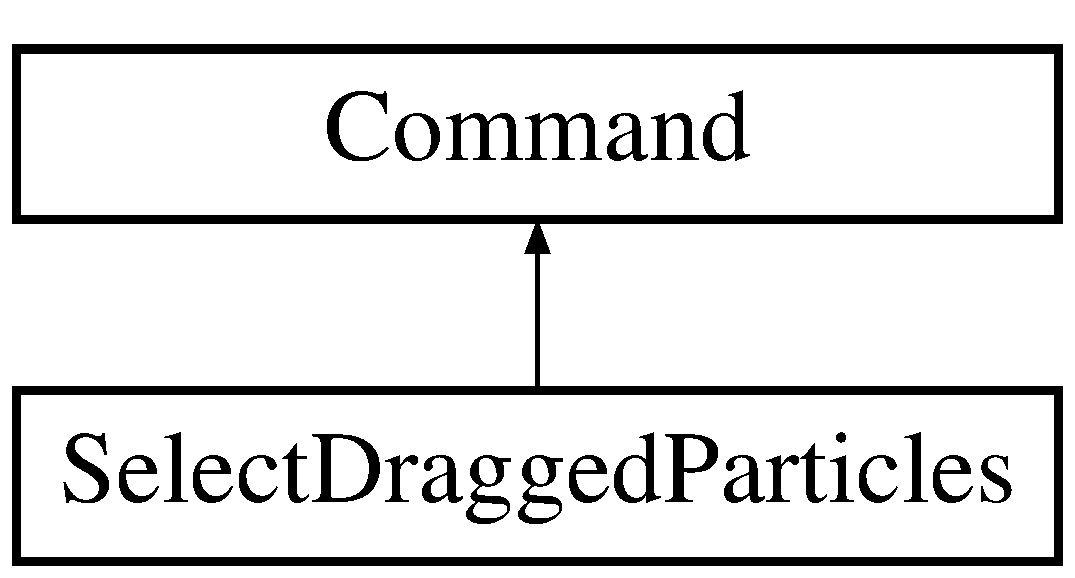
\includegraphics[height=2.000000cm]{classSelectDraggedParticles}
\end{center}
\end{figure}
\subsection*{Public Member Functions}
\begin{DoxyCompactItemize}
\item 
\hypertarget{classSelectDraggedParticles_a048c90d378429a3b19aa1c4696a31b0f}{void {\bfseries execute} ()}\label{classSelectDraggedParticles_a048c90d378429a3b19aa1c4696a31b0f}

\item 
\hypertarget{classSelectDraggedParticles_abece54f7450b0f91e7f0e4c1fead266b}{void {\bfseries setxy} (int \-\_\-x, int \-\_\-y)}\label{classSelectDraggedParticles_abece54f7450b0f91e7f0e4c1fead266b}

\end{DoxyCompactItemize}
\subsection*{Additional Inherited Members}


The documentation for this class was generated from the following file\-:\begin{DoxyCompactItemize}
\item 
include/\hyperlink{Commands_8h}{Commands.\-h}\end{DoxyCompactItemize}

\hypertarget{classSet3D}{\section{Set3\-D Class Reference}
\label{classSet3D}\index{Set3\-D@{Set3\-D}}
}
Inheritance diagram for Set3\-D\-:\begin{figure}[H]
\begin{center}
\leavevmode
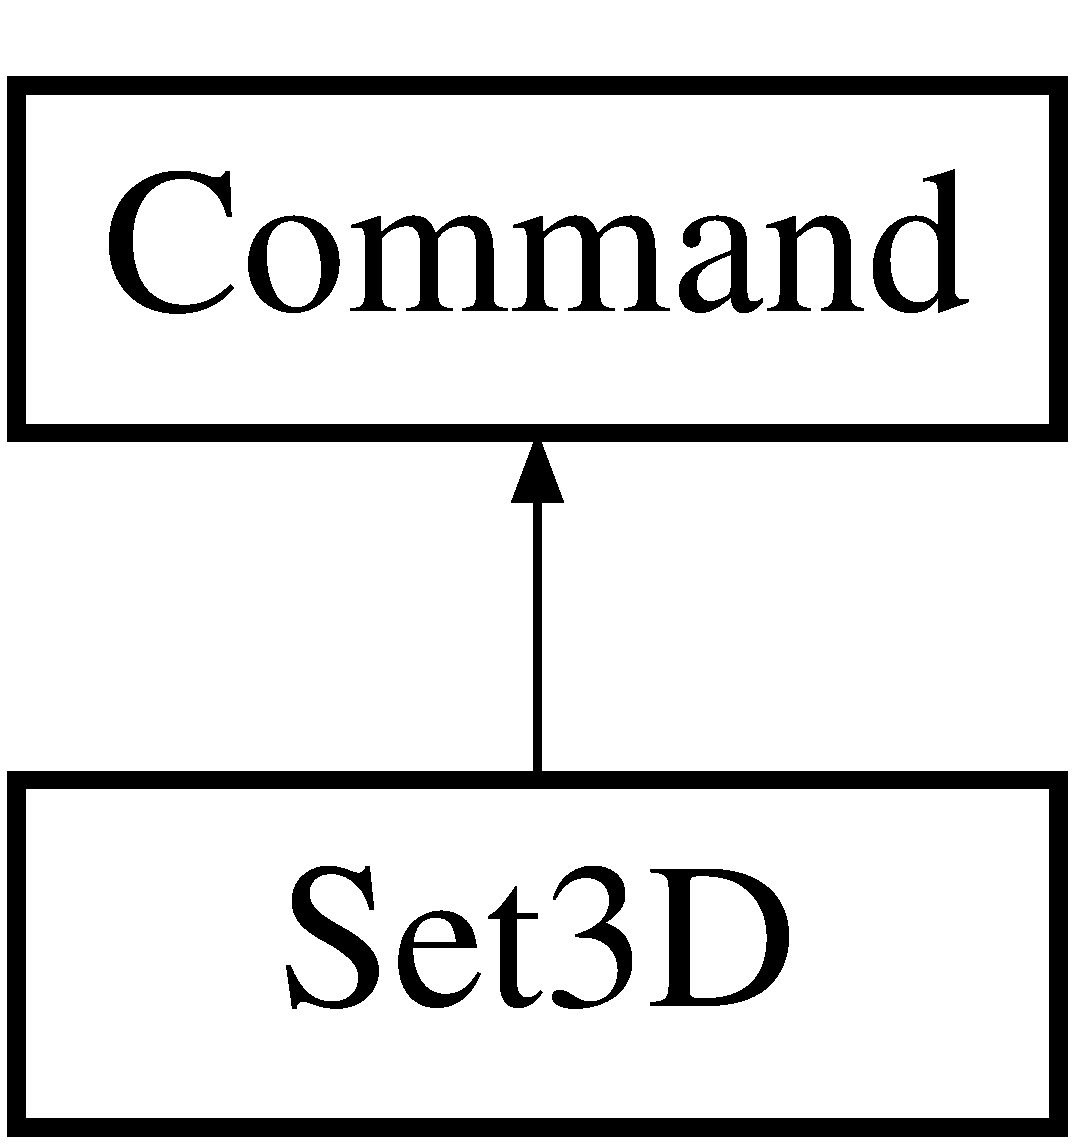
\includegraphics[height=2.000000cm]{classSet3D}
\end{center}
\end{figure}
\subsection*{Public Member Functions}
\begin{DoxyCompactItemize}
\item 
\hypertarget{classSet3D_a5862aab17e7e55c4a6a65fce27d8df74}{void {\bfseries execute} ()}\label{classSet3D_a5862aab17e7e55c4a6a65fce27d8df74}

\item 
\hypertarget{classSet3D_a10faf70f86f5dfe566e94a50f683b4f0}{void {\bfseries set\-Bool} (bool b)}\label{classSet3D_a10faf70f86f5dfe566e94a50f683b4f0}

\end{DoxyCompactItemize}
\subsection*{Additional Inherited Members}


The documentation for this class was generated from the following file\-:\begin{DoxyCompactItemize}
\item 
include/\hyperlink{Commands_8h}{Commands.\-h}\end{DoxyCompactItemize}

\hypertarget{structParticle_1_1spring}{\section{Particle\-:\-:spring Struct Reference}
\label{structParticle_1_1spring}\index{Particle\-::spring@{Particle\-::spring}}
}
\subsection*{Public Attributes}
\begin{DoxyCompactItemize}
\item 
\hypertarget{structParticle_1_1spring_a87a1c45bc8e6fda4fc24f973451d7374}{int {\bfseries indexi}}\label{structParticle_1_1spring_a87a1c45bc8e6fda4fc24f973451d7374}

\item 
\hypertarget{structParticle_1_1spring_a680b59e2d6ca1039267fc51b113c53a6}{int {\bfseries indexj}}\label{structParticle_1_1spring_a680b59e2d6ca1039267fc51b113c53a6}

\item 
\hypertarget{structParticle_1_1spring_a7bf4309301c1a087a79e7649ecd7185f}{G\-Lfloat {\bfseries L}}\label{structParticle_1_1spring_a7bf4309301c1a087a79e7649ecd7185f}

\item 
\hypertarget{structParticle_1_1spring_a9907abe5b485b2cead0fd23fd2d0d203}{int {\bfseries count}}\label{structParticle_1_1spring_a9907abe5b485b2cead0fd23fd2d0d203}

\item 
\hypertarget{structParticle_1_1spring_a35309948fe14fc48a7d428c75f6626e8}{bool {\bfseries alive}}\label{structParticle_1_1spring_a35309948fe14fc48a7d428c75f6626e8}

\end{DoxyCompactItemize}


The documentation for this struct was generated from the following file\-:\begin{DoxyCompactItemize}
\item 
include/\hyperlink{Particle_8h}{Particle.\-h}\end{DoxyCompactItemize}

\hypertarget{classToolbar}{\section{Toolbar Class Reference}
\label{classToolbar}\index{Toolbar@{Toolbar}}
}
\subsection*{Public Member Functions}
\begin{DoxyCompactItemize}
\item 
void \hyperlink{classToolbar_a0f068e7ccd28541382e1acee17450526}{draw\-Toolbar} (int \-\_\-h) const 
\begin{DoxyCompactList}\small\item\em draw\-Toolbar draws the toolbar on screen \end{DoxyCompactList}\item 
bool \hyperlink{classToolbar_a56977a2f551139471efd88a1ff471ccd}{handle\-Click\-Down} (int \-\_\-x, int \-\_\-y, int \-\_\-\-W\-I\-D\-T\-H, int \-\_\-\-H\-E\-I\-G\-H\-T)
\begin{DoxyCompactList}\small\item\em handle\-Click\-Down handles click on the toolbar \end{DoxyCompactList}\item 
\hypertarget{classToolbar_af9d231b63616a033490e8ac8d0c9f33b}{void \hyperlink{classToolbar_af9d231b63616a033490e8ac8d0c9f33b}{handle\-Click\-Up} ()}\label{classToolbar_af9d231b63616a033490e8ac8d0c9f33b}

\begin{DoxyCompactList}\small\item\em handle\-Click\-Up used when toolbar button only recesses while clicked down \end{DoxyCompactList}\item 
void \hyperlink{classToolbar_ac6227f656f1e27e143e4d0fd34df85cd}{handle\-Click\-Drop\-Down} (int \-\_\-x, int \-\_\-y, int \-\_\-\-W\-I\-D\-T\-H, int \-\_\-\-H\-E\-I\-G\-H\-T)
\begin{DoxyCompactList}\small\item\em handle\-Click\-Drop\-Down handles clicks on the dropdown menu \end{DoxyCompactList}\item 
void \hyperlink{classToolbar_a742772fb36768a80c2998cf135c65022}{toggle\-Bool} (bool $\ast$io\-\_\-toggleme)
\begin{DoxyCompactList}\small\item\em toggle\-Bool toggles the bool \end{DoxyCompactList}\item 
\hypertarget{classToolbar_a0d364406eeb8b7233850308b0eaf9a59}{bool {\bfseries get\-Drag} ()}\label{classToolbar_a0d364406eeb8b7233850308b0eaf9a59}

\item 
\hypertarget{classToolbar_a6a2b3c1096e6fca0096cd925ed4dc683}{bool {\bfseries get\-Draw} ()}\label{classToolbar_a6a2b3c1096e6fca0096cd925ed4dc683}

\item 
\hypertarget{classToolbar_ad857b74648d0d4f2efd6f97db0ee54bb}{bool {\bfseries get\-Help} ()}\label{classToolbar_ad857b74648d0d4f2efd6f97db0ee54bb}

\item 
\hypertarget{classToolbar_aa0f40959ba3b7aa73914493c80e8ea1c}{bool {\bfseries get\-Erase} ()}\label{classToolbar_aa0f40959ba3b7aa73914493c80e8ea1c}

\item 
bool \hyperlink{classToolbar_a999463c6c8f43502c201f36967c2dd74}{getdropdownopen} ()
\begin{DoxyCompactList}\small\item\em getdropdownopen returns bool saying whether the dropdown menu is open \end{DoxyCompactList}\item 
void \hyperlink{classToolbar_af7abc15cc148a86e52fd2b50b6486af3}{set\-World} (\hyperlink{classWorld}{World} $\ast$\-\_\-world)
\begin{DoxyCompactList}\small\item\em set\-World sets m\-\_\-world to the pointer input \end{DoxyCompactList}\item 
\hypertarget{classToolbar_a9ff9b46b71c99272a45bd867a8f67f11}{void {\bfseries press\-Draw} ()}\label{classToolbar_a9ff9b46b71c99272a45bd867a8f67f11}

\item 
\hypertarget{classToolbar_af276c240324605f344af36e09d051428}{void {\bfseries press\-Drag} ()}\label{classToolbar_af276c240324605f344af36e09d051428}

\item 
\hypertarget{classToolbar_ac5f6b68ddb0583c6cb8eeb7c0bf6f864}{void {\bfseries press\-Erase} ()}\label{classToolbar_ac5f6b68ddb0583c6cb8eeb7c0bf6f864}

\item 
\hypertarget{classToolbar_a0b5586c39a0b2994944bdcb20143ef5e}{void {\bfseries press\-Gravity} ()}\label{classToolbar_a0b5586c39a0b2994944bdcb20143ef5e}

\item 
\hypertarget{classToolbar_abb5720efecaf06bf139d45d62914b457}{void {\bfseries press\-Clear} ()}\label{classToolbar_abb5720efecaf06bf139d45d62914b457}

\item 
\hypertarget{classToolbar_ae0e45861a4a792c352ca409cd31e09fc}{void {\bfseries press\-Help} ()}\label{classToolbar_ae0e45861a4a792c352ca409cd31e09fc}

\item 
\hypertarget{classToolbar_a14b00fa84391b1a775b692ac33a886da}{void {\bfseries press\-Tap} ()}\label{classToolbar_a14b00fa84391b1a775b692ac33a886da}

\item 
\hypertarget{classToolbar_a38bf8d832bdc85b8474ca6dcf6cdbcd4}{void {\bfseries press\-Drop\-Down\-Menu} ()}\label{classToolbar_a38bf8d832bdc85b8474ca6dcf6cdbcd4}

\item 
\hypertarget{classToolbar_af61099a07fe60802002f80b74fadb32d}{void {\bfseries press\-Randomize} ()}\label{classToolbar_af61099a07fe60802002f80b74fadb32d}

\item 
\hypertarget{classToolbar_a67f52139298893d14adad059fed72cb6}{void {\bfseries press\-Camera} ()}\label{classToolbar_a67f52139298893d14adad059fed72cb6}

\item 
\hypertarget{classToolbar_a30ec2b7200f4ca7b9b9a603288a4ed21}{void \hyperlink{classToolbar_a30ec2b7200f4ca7b9b9a603288a4ed21}{remove\-Number} ()}\label{classToolbar_a30ec2b7200f4ca7b9b9a603288a4ed21}

\begin{DoxyCompactList}\small\item\em remove\-Number removes number from the seed for the randomised particle \end{DoxyCompactList}\item 
void \hyperlink{classToolbar_a8d529f805892e11052635ab1b95d453d}{draw\-Numbers} (float \-\_\-x, float \-\_\-y, int \-\_\-h, std\-::string \-\_\-numbers) const 
\begin{DoxyCompactList}\small\item\em draw\-Numbers draws the random seed numbers on screen \end{DoxyCompactList}\item 
void \hyperlink{classToolbar_a5563bdb5e874e1f2a0101dfd6e927941}{handle\-Keys} (char \-\_\-input)
\begin{DoxyCompactList}\small\item\em handle\-Keys makes sure relevant keys affect the toolbar buttons \end{DoxyCompactList}\item 
void \hyperlink{classToolbar_ab0051a6c70fad118c997b7d72e85d34f}{add\-Number} (char p)
\begin{DoxyCompactList}\small\item\em add\-Number adds number to the random seed (in char form) \end{DoxyCompactList}\item 
\hypertarget{classToolbar_aeb833afffead641813da1eec98f0bcad}{void {\bfseries draw\-Help\-Screen} () const }\label{classToolbar_aeb833afffead641813da1eec98f0bcad}

\end{DoxyCompactItemize}


\subsection{Member Function Documentation}
\hypertarget{classToolbar_ab0051a6c70fad118c997b7d72e85d34f}{\index{Toolbar@{Toolbar}!add\-Number@{add\-Number}}
\index{add\-Number@{add\-Number}!Toolbar@{Toolbar}}
\subsubsection[{add\-Number}]{\setlength{\rightskip}{0pt plus 5cm}void Toolbar\-::add\-Number (
\begin{DoxyParamCaption}
\item[{char}]{p}
\end{DoxyParamCaption}
)}}\label{classToolbar_ab0051a6c70fad118c997b7d72e85d34f}


add\-Number adds number to the random seed (in char form) 


\begin{DoxyParams}[1]{Parameters}
\mbox{\tt in}  & {\em \-\_\-p} & character to add \\
\hline
\end{DoxyParams}
\hypertarget{classToolbar_a8d529f805892e11052635ab1b95d453d}{\index{Toolbar@{Toolbar}!draw\-Numbers@{draw\-Numbers}}
\index{draw\-Numbers@{draw\-Numbers}!Toolbar@{Toolbar}}
\subsubsection[{draw\-Numbers}]{\setlength{\rightskip}{0pt plus 5cm}void Toolbar\-::draw\-Numbers (
\begin{DoxyParamCaption}
\item[{float}]{\-\_\-x, }
\item[{float}]{\-\_\-y, }
\item[{int}]{\-\_\-h, }
\item[{std\-::string}]{\-\_\-numbers}
\end{DoxyParamCaption}
) const}}\label{classToolbar_a8d529f805892e11052635ab1b95d453d}


draw\-Numbers draws the random seed numbers on screen 


\begin{DoxyParams}[1]{Parameters}
\mbox{\tt in}  & {\em \-\_\-x} & x coordinate of mouse on screen in pixels \\
\hline
\mbox{\tt in}  & {\em \-\_\-y} & y coordinate of mouse on screen in pixels \\
\hline
\mbox{\tt in}  & {\em \-\_\-h} & height of window in pixels \\
\hline
\mbox{\tt in}  & {\em \-\_\-numbers} & numbers to draw \\
\hline
\end{DoxyParams}
\hypertarget{classToolbar_a0f068e7ccd28541382e1acee17450526}{\index{Toolbar@{Toolbar}!draw\-Toolbar@{draw\-Toolbar}}
\index{draw\-Toolbar@{draw\-Toolbar}!Toolbar@{Toolbar}}
\subsubsection[{draw\-Toolbar}]{\setlength{\rightskip}{0pt plus 5cm}void Toolbar\-::draw\-Toolbar (
\begin{DoxyParamCaption}
\item[{int}]{\-\_\-h}
\end{DoxyParamCaption}
) const}}\label{classToolbar_a0f068e7ccd28541382e1acee17450526}


draw\-Toolbar draws the toolbar on screen 


\begin{DoxyParams}{Parameters}
{\em \-\_\-h} & window height in pixels \\
\hline
\end{DoxyParams}
\hypertarget{classToolbar_a999463c6c8f43502c201f36967c2dd74}{\index{Toolbar@{Toolbar}!getdropdownopen@{getdropdownopen}}
\index{getdropdownopen@{getdropdownopen}!Toolbar@{Toolbar}}
\subsubsection[{getdropdownopen}]{\setlength{\rightskip}{0pt plus 5cm}bool Toolbar\-::getdropdownopen (
\begin{DoxyParamCaption}
{}
\end{DoxyParamCaption}
)}}\label{classToolbar_a999463c6c8f43502c201f36967c2dd74}


getdropdownopen returns bool saying whether the dropdown menu is open 

\begin{DoxyReturn}{Returns}
bool saying whether the dropdown menu is open 
\end{DoxyReturn}
\hypertarget{classToolbar_a56977a2f551139471efd88a1ff471ccd}{\index{Toolbar@{Toolbar}!handle\-Click\-Down@{handle\-Click\-Down}}
\index{handle\-Click\-Down@{handle\-Click\-Down}!Toolbar@{Toolbar}}
\subsubsection[{handle\-Click\-Down}]{\setlength{\rightskip}{0pt plus 5cm}bool Toolbar\-::handle\-Click\-Down (
\begin{DoxyParamCaption}
\item[{int}]{\-\_\-x, }
\item[{int}]{\-\_\-y, }
\item[{int}]{\-\_\-\-W\-I\-D\-T\-H, }
\item[{int}]{\-\_\-\-H\-E\-I\-G\-H\-T}
\end{DoxyParamCaption}
)}}\label{classToolbar_a56977a2f551139471efd88a1ff471ccd}


handle\-Click\-Down handles click on the toolbar 


\begin{DoxyParams}[1]{Parameters}
\mbox{\tt in}  & {\em \-\_\-x} & x coordinate of mouse on screen in pixels \\
\hline
\mbox{\tt in}  & {\em \-\_\-y} & y coordinate of mouse on screen in pixels \\
\hline
\mbox{\tt in}  & {\em \-\_\-\-W\-I\-D\-T\-H} & width of window in pixels \\
\hline
\mbox{\tt in}  & {\em \-\_\-\-H\-E\-I\-G\-H\-T} & height of window in pixels \\
\hline
\end{DoxyParams}
\begin{DoxyReturn}{Returns}
if click is on screen returns true else false 
\end{DoxyReturn}
\hypertarget{classToolbar_ac6227f656f1e27e143e4d0fd34df85cd}{\index{Toolbar@{Toolbar}!handle\-Click\-Drop\-Down@{handle\-Click\-Drop\-Down}}
\index{handle\-Click\-Drop\-Down@{handle\-Click\-Drop\-Down}!Toolbar@{Toolbar}}
\subsubsection[{handle\-Click\-Drop\-Down}]{\setlength{\rightskip}{0pt plus 5cm}void Toolbar\-::handle\-Click\-Drop\-Down (
\begin{DoxyParamCaption}
\item[{int}]{\-\_\-x, }
\item[{int}]{\-\_\-y, }
\item[{int}]{\-\_\-\-W\-I\-D\-T\-H, }
\item[{int}]{\-\_\-\-H\-E\-I\-G\-H\-T}
\end{DoxyParamCaption}
)}}\label{classToolbar_ac6227f656f1e27e143e4d0fd34df85cd}


handle\-Click\-Drop\-Down handles clicks on the dropdown menu 


\begin{DoxyParams}[1]{Parameters}
\mbox{\tt in}  & {\em \-\_\-x} & x coordinate of mouse on screen in pixels \\
\hline
\mbox{\tt in}  & {\em \-\_\-y} & y coordinate of mouse on screen in pixels \\
\hline
\mbox{\tt in}  & {\em \-\_\-\-W\-I\-D\-T\-H} & width of window in pixels \\
\hline
\mbox{\tt in}  & {\em \-\_\-\-H\-E\-I\-G\-H\-T} & height of window in pixels \\
\hline
\end{DoxyParams}
\hypertarget{classToolbar_a5563bdb5e874e1f2a0101dfd6e927941}{\index{Toolbar@{Toolbar}!handle\-Keys@{handle\-Keys}}
\index{handle\-Keys@{handle\-Keys}!Toolbar@{Toolbar}}
\subsubsection[{handle\-Keys}]{\setlength{\rightskip}{0pt plus 5cm}void Toolbar\-::handle\-Keys (
\begin{DoxyParamCaption}
\item[{char}]{\-\_\-input}
\end{DoxyParamCaption}
)}}\label{classToolbar_a5563bdb5e874e1f2a0101dfd6e927941}


handle\-Keys makes sure relevant keys affect the toolbar buttons 


\begin{DoxyParams}[1]{Parameters}
\mbox{\tt in}  & {\em \-\_\-input} & the character to handle \\
\hline
\end{DoxyParams}
\hypertarget{classToolbar_af7abc15cc148a86e52fd2b50b6486af3}{\index{Toolbar@{Toolbar}!set\-World@{set\-World}}
\index{set\-World@{set\-World}!Toolbar@{Toolbar}}
\subsubsection[{set\-World}]{\setlength{\rightskip}{0pt plus 5cm}void Toolbar\-::set\-World (
\begin{DoxyParamCaption}
\item[{{\bf World} $\ast$}]{\-\_\-world}
\end{DoxyParamCaption}
)}}\label{classToolbar_af7abc15cc148a86e52fd2b50b6486af3}


set\-World sets m\-\_\-world to the pointer input 


\begin{DoxyParams}[1]{Parameters}
\mbox{\tt in}  & {\em \-\_\-world} & the pointer to set m\-\_\-world to \\
\hline
\end{DoxyParams}
\hypertarget{classToolbar_a742772fb36768a80c2998cf135c65022}{\index{Toolbar@{Toolbar}!toggle\-Bool@{toggle\-Bool}}
\index{toggle\-Bool@{toggle\-Bool}!Toolbar@{Toolbar}}
\subsubsection[{toggle\-Bool}]{\setlength{\rightskip}{0pt plus 5cm}void Toolbar\-::toggle\-Bool (
\begin{DoxyParamCaption}
\item[{bool $\ast$}]{io\-\_\-toggleme}
\end{DoxyParamCaption}
)}}\label{classToolbar_a742772fb36768a80c2998cf135c65022}


toggle\-Bool toggles the bool 


\begin{DoxyParams}[1]{Parameters}
\mbox{\tt in,out}  & {\em io\-\_\-toggleme} & pointer to the bool to toggle \\
\hline
\end{DoxyParams}


The documentation for this class was generated from the following file\-:\begin{DoxyCompactItemize}
\item 
include/\hyperlink{Toolbar_8h}{Toolbar.\-h}\end{DoxyCompactItemize}

\hypertarget{classVec3}{\section{Vec3 Class Reference}
\label{classVec3}\index{Vec3@{Vec3}}
}
\subsection*{Public Member Functions}
\begin{DoxyCompactItemize}
\item 
\hypertarget{classVec3_a42149bc6fb27116cec34c0bf9d41b096}{{\bfseries Vec3} (const \hyperlink{classVec3}{Vec3} \&\-\_\-rhs)=default}\label{classVec3_a42149bc6fb27116cec34c0bf9d41b096}

\item 
\hypertarget{classVec3_a430e79b181cdcf9fb2b0459d9d609563}{{\bfseries Vec3} (G\-Lfloat \-\_\-x=0.\-0f, G\-Lfloat \-\_\-y=0.\-0f, G\-Lfloat \-\_\-z=0.\-0f)}\label{classVec3_a430e79b181cdcf9fb2b0459d9d609563}

\item 
\hypertarget{classVec3_a033d1bb50bc8c3e5d03bb90242f671dc}{float {\bfseries dot} (const \hyperlink{classVec3}{Vec3} \&\-\_\-rhs) const }\label{classVec3_a033d1bb50bc8c3e5d03bb90242f671dc}

\item 
\hypertarget{classVec3_a17b354d08f44a6cad8e435aea73ae7f9}{float {\bfseries length} () const }\label{classVec3_a17b354d08f44a6cad8e435aea73ae7f9}

\item 
\hypertarget{classVec3_af34508ce91419757caf6481c654dc08b}{float {\bfseries length\-Squared} () const }\label{classVec3_af34508ce91419757caf6481c654dc08b}

\item 
\hypertarget{classVec3_a3a6631559d1d36eaf34ca586ce86ede1}{void {\bfseries normalize} ()}\label{classVec3_a3a6631559d1d36eaf34ca586ce86ede1}

\item 
\hypertarget{classVec3_a0914b708a219db3d38ff2fcc1d8a766e}{\hyperlink{classVec3}{Vec3} {\bfseries cross} (\hyperlink{classVec3}{Vec3} \&\-\_\-rhs) const }\label{classVec3_a0914b708a219db3d38ff2fcc1d8a766e}

\item 
\hypertarget{classVec3_a425331dd9d20a3a9b9354303e7fa7ad1}{void {\bfseries rotate\-Around\-X\-Axisf} (float degrees)}\label{classVec3_a425331dd9d20a3a9b9354303e7fa7ad1}

\item 
\hypertarget{classVec3_a3ebcf5f1fb0f9a7ffd511d958d78fd91}{\hyperlink{classVec3}{Vec3} {\bfseries operator$\ast$} (\hyperlink{classMat3}{Mat3} \&\-\_\-rhs)}\label{classVec3_a3ebcf5f1fb0f9a7ffd511d958d78fd91}

\item 
\hypertarget{classVec3_a46ffb589de4804e6e6d37dea9c5a22b4}{\hyperlink{classVec3}{Vec3} {\bfseries operator$\ast$} (G\-Lfloat \-\_\-rhs) const }\label{classVec3_a46ffb589de4804e6e6d37dea9c5a22b4}

\item 
\hypertarget{classVec3_a678d1234531fdb6863a7171ea9cadd49}{void {\bfseries operator$\ast$=} (G\-Lfloat \-\_\-rhs)}\label{classVec3_a678d1234531fdb6863a7171ea9cadd49}

\item 
\hypertarget{classVec3_afadfe01be0d872aa61920c37f19eb9a4}{\hyperlink{classVec3}{Vec3} {\bfseries operator/} (G\-Lfloat \-\_\-rhs) const }\label{classVec3_afadfe01be0d872aa61920c37f19eb9a4}

\item 
\hypertarget{classVec3_a10db8b8877035b44b29df695f08b17ca}{void {\bfseries operator/=} (G\-Lfloat \-\_\-rhs)}\label{classVec3_a10db8b8877035b44b29df695f08b17ca}

\item 
\hypertarget{classVec3_af4bf43738408bc28c2298df99a420910}{\hyperlink{classVec3}{Vec3} {\bfseries operator+} (const \hyperlink{classVec3}{Vec3} \&\-\_\-r) const }\label{classVec3_af4bf43738408bc28c2298df99a420910}

\item 
\hypertarget{classVec3_a66d0477871d90a8ab7fe4fb903657ac3}{void {\bfseries operator+=} (const \hyperlink{classVec3}{Vec3} \&\-\_\-r)}\label{classVec3_a66d0477871d90a8ab7fe4fb903657ac3}

\item 
\hypertarget{classVec3_a1af6ff2a6a2c71bfe6f832ef61923edd}{\hyperlink{classVec3}{Vec3} {\bfseries operator-\/} (const \hyperlink{classVec3}{Vec3} \&\-\_\-rhs) const }\label{classVec3_a1af6ff2a6a2c71bfe6f832ef61923edd}

\item 
\hypertarget{classVec3_aab77f0f572c56fdee062228fe9b02242}{\hyperlink{classVec3}{Vec3} {\bfseries operator-\/} ()}\label{classVec3_aab77f0f572c56fdee062228fe9b02242}

\item 
\hypertarget{classVec3_ac6a5efb269a181d7b0e7a6a350f3cd20}{void {\bfseries operator-\/=} (const \hyperlink{classVec3}{Vec3} \&\-\_\-r)}\label{classVec3_ac6a5efb269a181d7b0e7a6a350f3cd20}

\item 
\hypertarget{classVec3_a9b41ea429d7d6407df1edd5aac5fa0e6}{bool {\bfseries operator==} (const \hyperlink{classVec3}{Vec3} \&\-\_\-rhs) const }\label{classVec3_a9b41ea429d7d6407df1edd5aac5fa0e6}

\item 
\hypertarget{classVec3_a9cab569511fddfcf377dc21ffdae4693}{G\-Lfloat \& {\bfseries operator\mbox{[}$\,$\mbox{]}} (int \-\_\-i)}\label{classVec3_a9cab569511fddfcf377dc21ffdae4693}

\item 
\hypertarget{classVec3_ac1b15d91c3a8735d411d54eb7baba015}{void {\bfseries set} (G\-Lfloat \-\_\-x, G\-Lfloat \-\_\-y, G\-Lfloat \-\_\-z)}\label{classVec3_ac1b15d91c3a8735d411d54eb7baba015}

\item 
\hypertarget{classVec3_a3f151676ea36dc9e6047489dd76de2be}{void {\bfseries vertex\-G\-L} () const }\label{classVec3_a3f151676ea36dc9e6047489dd76de2be}

\end{DoxyCompactItemize}


The documentation for this class was generated from the following file\-:\begin{DoxyCompactItemize}
\item 
include/\hyperlink{Vec3_8h}{Vec3.\-h}\end{DoxyCompactItemize}

\hypertarget{classWorld}{\section{World Class Reference}
\label{classWorld}\index{World@{World}}
}


The Scene class.  




{\ttfamily \#include $<$World.\-h$>$}

\subsection*{Public Member Functions}
\begin{DoxyCompactItemize}
\item 
\hypertarget{classWorld_afa39d4e6f714a7a3691ac0c656f5e8a8}{\hyperlink{classWorld_afa39d4e6f714a7a3691ac0c656f5e8a8}{World} ()}\label{classWorld_afa39d4e6f714a7a3691ac0c656f5e8a8}

\begin{DoxyCompactList}\small\item\em A constructor, called when this class is instanced in the form of an object. \end{DoxyCompactList}\item 
\hypertarget{classWorld_a8c73fba541a5817fff65147ba47cd827}{\hyperlink{classWorld_a8c73fba541a5817fff65147ba47cd827}{$\sim$\-World} ()}\label{classWorld_a8c73fba541a5817fff65147ba47cd827}

\begin{DoxyCompactList}\small\item\em A virtual destructor, in case we want to inherit from this class. \end{DoxyCompactList}\item 
\hypertarget{classWorld_a0150607a49c2400d5c848159dd02d533}{void \hyperlink{classWorld_a0150607a49c2400d5c848159dd02d533}{init} ()}\label{classWorld_a0150607a49c2400d5c848159dd02d533}

\begin{DoxyCompactList}\small\item\em init Initialises the scene, called before render(). \end{DoxyCompactList}\item 
void \hyperlink{classWorld_aed4b52aa267ebcebe7087119529639f3}{resize\-World} (int \-\_\-w, int \-\_\-h)
\begin{DoxyCompactList}\small\item\em resize\-World resizes the spatial hash and world objects when window size changes \end{DoxyCompactList}\item 
void \hyperlink{classWorld_a64d27720442ce140c8095566e8035b54}{resize\-Window} (int \-\_\-w, int \-\_\-h)
\begin{DoxyCompactList}\small\item\em resize\-Window resizes the S\-D\-L window \& Open\-G\-L \end{DoxyCompactList}\item 
void \hyperlink{classWorld_ab3f32d708c9f53e337f8352ac3b0641d}{update} (bool $\ast$o\-\_\-updateinprogress)
\begin{DoxyCompactList}\small\item\em update updates the particles in the world according to S\-P\-H algorithms. Called in timer. \end{DoxyCompactList}\item 
\hypertarget{classWorld_ab51a17ccbb108616daacd0c34973dc8d}{void \hyperlink{classWorld_ab51a17ccbb108616daacd0c34973dc8d}{draw} ()}\label{classWorld_ab51a17ccbb108616daacd0c34973dc8d}

\begin{DoxyCompactList}\small\item\em draw Draws the particles in the world either in spheres, marching cubes or squares \end{DoxyCompactList}\item 
float \hyperlink{classWorld_abf6fa37003722e1fba8862f6eb299c2d}{get\-Half\-Height} () const 
\begin{DoxyCompactList}\small\item\em get\-Half\-Height returns half the height of the window in Open\-G\-L coordinates \end{DoxyCompactList}\item 
float \hyperlink{classWorld_a68605fd591772396a7ffbc3dcc1802a2}{get\-Half\-Width} () const 
\begin{DoxyCompactList}\small\item\em get\-Half\-Width returns half the width of the window in Open\-G\-L coordinates \end{DoxyCompactList}\item 
\hyperlink{classVec3}{Vec3} \hyperlink{classWorld_ae87279ec231161c8e41f1839f47c8dac}{get\-Grid\-Column\-Row} (int \-\_\-k)
\begin{DoxyCompactList}\small\item\em get\-Grid\-Column\-Row returns the grid's column and row number from the spatial hash number \end{DoxyCompactList}\item 
std\-::vector$<$ \hyperlink{classParticle}{Particle} $\ast$ $>$ \hyperlink{classWorld_a0c93ff0f6b57f9f45160e3fc985f318f}{get\-Surrounding\-Particles} (int thiscell, int numsur, bool withwalls) const 
\begin{DoxyCompactList}\small\item\em get\-Surrounding\-Particles gets all particles in surrounding grids. \end{DoxyCompactList}\item 
void \hyperlink{classWorld_a0847c4e3dc1a17791949ac49aaba449b}{getbackhere} (\hyperlink{classParticle}{Particle} $\ast$io\-\_\-p)
\begin{DoxyCompactList}\small\item\em getbackhere if particle is out of boundaries then it's position is changes so it is within boundaries \end{DoxyCompactList}\item 
void \hyperlink{classWorld_a738c729dace44a14ec64529eb47aae3b}{handle\-Keys} (char \-\_\-input)
\begin{DoxyCompactList}\small\item\em handle\-Keys handles keyboard key inputs that affect the particles within the world \end{DoxyCompactList}\item 
void \hyperlink{classWorld_a5b90e83051311490ea6e9a7862cb7aae}{delete\-Spring} (int \-\_\-s)
\begin{DoxyCompactList}\small\item\em delete\-Spring deletes a spring from the vector m\-\_\-springs while updating m\-\_\-last\-Free\-Spring and m\-\_\-last\-Taken\-Spring \end{DoxyCompactList}\item 
int \hyperlink{classWorld_ad28f7d1bd3a6b181513ce92d0b76a9d6}{insert\-Spring} (\hyperlink{structParticle_1_1spring}{Particle\-::\-Spring} \-\_\-spring)
\begin{DoxyCompactList}\small\item\em insert\-Spring Inserts a spring to the vector m\-\_\-springs while updating m\-\_\-last\-Free\-Spring and m\-\_\-last\-Taken\-Spring \end{DoxyCompactList}\item 
void \hyperlink{classWorld_ae1850c34d62127f1864c0c031e882c63}{delete\-Particle} (int \-\_\-p)
\begin{DoxyCompactList}\small\item\em delete\-Particle deletes a particle from the vector m\-\_\-particles while updating m\-\_\-last\-Free\-Particle and m\-\_\-last\-Taken\-Particle \end{DoxyCompactList}\item 
void \hyperlink{classWorld_aa962526ce57792d47848c5dc24530097}{insert\-Particle} (\hyperlink{classParticle}{Particle} \-\_\-particle)
\begin{DoxyCompactList}\small\item\em insert\-Particle inserts a particle to the vector m\-\_\-particles while updating m\-\_\-last\-Free\-Particle and m\-\_\-last\-Taken\-Particle \end{DoxyCompactList}\item 
\hypertarget{classWorld_abf37c2bf5e92f910a963153f46f9af41}{void \hyperlink{classWorld_abf37c2bf5e92f910a963153f46f9af41}{defrag\-Particles} ()}\label{classWorld_abf37c2bf5e92f910a963153f46f9af41}

\begin{DoxyCompactList}\small\item\em defrag\-Particles reorders the particles within m\-\_\-particles so all alive particles are to the left \end{DoxyCompactList}\item 
\hypertarget{classWorld_a3036437a8edfd623efa899e1ee9438a0}{void \hyperlink{classWorld_a3036437a8edfd623efa899e1ee9438a0}{defrag\-Springs} ()}\label{classWorld_a3036437a8edfd623efa899e1ee9438a0}

\begin{DoxyCompactList}\small\item\em defrag\-Springs reorders the springs within m\-\_\-springs so that all alive springs are to the left \end{DoxyCompactList}\item 
\hypertarget{classWorld_ae27fe9607ae7b01b911568759862bbd5}{void \hyperlink{classWorld_ae27fe9607ae7b01b911568759862bbd5}{hash\-Particles} ()}\label{classWorld_ae27fe9607ae7b01b911568759862bbd5}

\begin{DoxyCompactList}\small\item\em hash\-Particles takes m\-\_\-grid and m\-\_\-particles, using spatial hash organises the particles into buckets / squares as pointers \end{DoxyCompactList}\item 
\hypertarget{classWorld_aae7e186e5bfedcc4c119346733de2a80}{bool {\bfseries is\-Left\-Button\-Pressed} ()}\label{classWorld_aae7e186e5bfedcc4c119346733de2a80}

\item 
\hypertarget{classWorld_a28f2d9a8e63dd01cca8dc7c102457fc6}{void {\bfseries mouse\-Draw} (int x, int y)}\label{classWorld_a28f2d9a8e63dd01cca8dc7c102457fc6}

\item 
\hypertarget{classWorld_a55549f4354974b87fc03759ce15ba7af}{void {\bfseries mouse\-Drag} (int x, int y)}\label{classWorld_a55549f4354974b87fc03759ce15ba7af}

\item 
\hypertarget{classWorld_a3a343bef6ff44293b3c394e50f711436}{void {\bfseries mouse\-Erase} (int x, int y)}\label{classWorld_a3a343bef6ff44293b3c394e50f711436}

\item 
\hypertarget{classWorld_aa2adabb735614bed42f0dcc6333e28b9}{void {\bfseries mouse\-Drag\-End} (int x, int y)}\label{classWorld_aa2adabb735614bed42f0dcc6333e28b9}

\item 
\hypertarget{classWorld_afb61fbb93e58ddda9acab26f67b2de26}{void {\bfseries select\-Dragged\-Particles} (int x, int y)}\label{classWorld_afb61fbb93e58ddda9acab26f67b2de26}

\item 
\hypertarget{classWorld_ae5cb0a8dd0696ed65284ce0e8560ddf5}{void {\bfseries toggle\-Rain} ()}\label{classWorld_ae5cb0a8dd0696ed65284ce0e8560ddf5}

\item 
\hypertarget{classWorld_aa8efd033209cbf9e0391f3adf1ddf4dc}{void {\bfseries toggle\-Gravity} ()}\label{classWorld_aa8efd033209cbf9e0391f3adf1ddf4dc}

\item 
\hypertarget{classWorld_aa6e788d15f389d634ccd1148f47cfb96}{void {\bfseries clear\-World} ()}\label{classWorld_aa6e788d15f389d634ccd1148f47cfb96}

\item 
\hypertarget{classWorld_a464e5e41c3cf428b4ac97b67c826c8eb}{void {\bfseries set3\-D} (bool b)}\label{classWorld_a464e5e41c3cf428b4ac97b67c826c8eb}

\item 
\hypertarget{classWorld_a561567c6a539a240f3ed54ff228f5271}{bool {\bfseries get3\-D} ()}\label{classWorld_a561567c6a539a240f3ed54ff228f5271}

\item 
\hypertarget{classWorld_a7eb707b21072c77214420804e662d906}{void {\bfseries draw\-With} (int type)}\label{classWorld_a7eb707b21072c77214420804e662d906}

\item 
\hypertarget{classWorld_a0cd51e0a2125d62aa76c29359785e0f5}{void {\bfseries mouse\-Move} (const int \&x, const int \&y, bool leftclick, bool rightclick)}\label{classWorld_a0cd51e0a2125d62aa76c29359785e0f5}

\item 
\hypertarget{classWorld_a6fcdae48d4867a7f42d7c49c57433ab3}{void {\bfseries drawchar} ()}\label{classWorld_a6fcdae48d4867a7f42d7c49c57433ab3}

\item 
\hypertarget{classWorld_a2306bf46e36020f35a7d3bc2527434fb}{void {\bfseries set\-To\-Draw} (int \-\_\-todraw)}\label{classWorld_a2306bf46e36020f35a7d3bc2527434fb}

\item 
\hypertarget{classWorld_aadab7988ffe1e55c10ad34f85199e385}{void {\bfseries set\-Random\-Type} (int \-\_\-random\-Seed)}\label{classWorld_aadab7988ffe1e55c10ad34f85199e385}

\item 
\hypertarget{classWorld_a37363e2d9fb17fa31691af105c6e6a8c}{void {\bfseries make\-Particles\-Big} ()}\label{classWorld_a37363e2d9fb17fa31691af105c6e6a8c}

\item 
\hypertarget{classWorld_a0c111bf57420a13120baca933b9f250f}{void {\bfseries make\-Particles\-Small} ()}\label{classWorld_a0c111bf57420a13120baca933b9f250f}

\item 
\hypertarget{classWorld_a4967d249f71084117a4b6a84a58dba9f}{std\-::vector$<$ std\-::vector$<$ float $>$ $>$ {\bfseries render\-Grid} (\hyperlink{classParticleProperties}{Particle\-Properties} $\ast$p)}\label{classWorld_a4967d249f71084117a4b6a84a58dba9f}

\item 
\hypertarget{classWorld_a119745daabbf33b5eea16f6c1fa13539}{std\-::vector$<$ std\-::vector\\*
$<$ std\-::vector$<$ float $>$ $>$ $>$ {\bfseries render3d\-Grid} (\hyperlink{classParticleProperties}{Particle\-Properties} $\ast$p)}\label{classWorld_a119745daabbf33b5eea16f6c1fa13539}

\item 
\hypertarget{classWorld_a79bfda3d3ee02e561f37fa3ef65e72ff}{\hyperlink{classVec3}{Vec3} {\bfseries get\-Grid\-X\-Y\-Z} (int k)}\label{classWorld_a79bfda3d3ee02e561f37fa3ef65e72ff}

\item 
\hypertarget{classWorld_a1a2aab6852fd79ee5d661ee45e2c3b7a}{int {\bfseries getrenderoption} ()}\label{classWorld_a1a2aab6852fd79ee5d661ee45e2c3b7a}

\item 
\hypertarget{classWorld_acdaeb9fef04e92b52562b630475e1553}{void {\bfseries draw\-Loading} ()}\label{classWorld_acdaeb9fef04e92b52562b630475e1553}

\item 
\hypertarget{classWorld_a557bf718ffb5976ae4a35daf526b6bbb}{void {\bfseries increase2\-D\-Resolution\-W\-O\-R\-L\-D} ()}\label{classWorld_a557bf718ffb5976ae4a35daf526b6bbb}

\item 
\hypertarget{classWorld_a7c0c14a57f64e4e3ffd5a5ef9f5c8156}{void {\bfseries decrease2\-D\-Resolution\-W\-O\-R\-L\-D} ()}\label{classWorld_a7c0c14a57f64e4e3ffd5a5ef9f5c8156}

\item 
\hypertarget{classWorld_a1d31371f414e6b21e584873aed9ccc22}{int {\bfseries get\-Snapshot\-Mode} ()}\label{classWorld_a1d31371f414e6b21e584873aed9ccc22}

\item 
\hypertarget{classWorld_ab035312321b021858d62e8235f8b9e02}{void {\bfseries draw\-Cube} ()}\label{classWorld_ab035312321b021858d62e8235f8b9e02}

\end{DoxyCompactItemize}
\subsection*{Protected Attributes}
\begin{DoxyCompactItemize}
\item 
\hypertarget{classWorld_a8d2c7904c78772cd416046f17e8fde9a}{bool \hyperlink{classWorld_a8d2c7904c78772cd416046f17e8fde9a}{m\-\_\-is\-Init}}\label{classWorld_a8d2c7904c78772cd416046f17e8fde9a}

\begin{DoxyCompactList}\small\item\em Keep track of whether this has been initialised -\/ otherwise it won't be ready to draw! \end{DoxyCompactList}\item 
\hypertarget{classWorld_aea913074e52f86a713d2fd2e3ab4c84f}{double \hyperlink{classWorld_aea913074e52f86a713d2fd2e3ab4c84f}{m\-\_\-start\-Time}}\label{classWorld_aea913074e52f86a713d2fd2e3ab4c84f}

\begin{DoxyCompactList}\small\item\em The time since the object was initialised, which is used for animation purposes. \end{DoxyCompactList}\item 
\hypertarget{classWorld_a96627a74533eb71253e347b1d5754380}{double \hyperlink{classWorld_a96627a74533eb71253e347b1d5754380}{m\-\_\-elapsed\-Time}}\label{classWorld_a96627a74533eb71253e347b1d5754380}

\begin{DoxyCompactList}\small\item\em A member that is updated when \hyperlink{classWorld_ab3f32d708c9f53e337f8352ac3b0641d}{update()} is called indicating the elapsed time. \end{DoxyCompactList}\item 
\hypertarget{classWorld_ac07d502be70b521c99aee1876919d5dd}{double {\bfseries m\-\_\-timestep}}\label{classWorld_ac07d502be70b521c99aee1876919d5dd}

\item 
\hypertarget{classWorld_a927cf4a925c2e45a5994fdf4ed935088}{std\-::vector$<$ \hyperlink{classParticle}{Particle} $>$ {\bfseries m\-\_\-particles}}\label{classWorld_a927cf4a925c2e45a5994fdf4ed935088}

\item 
\hypertarget{classWorld_a29c3c75f7459ce8fd396885cd2cf508d}{int {\bfseries m\-\_\-particles\-Pool\-Size}}\label{classWorld_a29c3c75f7459ce8fd396885cd2cf508d}

\item 
\hypertarget{classWorld_a8aa72ceb0053b37ebf3bfc9dfa3f7d67}{int {\bfseries m\-\_\-first\-Free\-Particle}}\label{classWorld_a8aa72ceb0053b37ebf3bfc9dfa3f7d67}

\item 
\hypertarget{classWorld_ac3a684ea22c602344a61fc3ff7c8f444}{int {\bfseries m\-\_\-last\-Taken\-Particle}}\label{classWorld_ac3a684ea22c602344a61fc3ff7c8f444}

\item 
\hypertarget{classWorld_a0e8bf89890e6e1874e53ed8db76e885c}{int {\bfseries m\-\_\-how\-Many\-Alive\-Particles}}\label{classWorld_a0e8bf89890e6e1874e53ed8db76e885c}

\item 
\hypertarget{classWorld_af3a83d8820ece274292746482991d9a0}{std\-::vector$<$ \hyperlink{classParticleProperties}{Particle\-Properties} $>$ {\bfseries m\-\_\-particle\-Types}}\label{classWorld_af3a83d8820ece274292746482991d9a0}

\item 
\hypertarget{classWorld_a4f43c7ae20726ca36a2438fc05dba9e6}{std\-::vector$<$ std\-::vector\\*
$<$ \hyperlink{classParticle}{Particle} $\ast$ $>$ $>$ {\bfseries m\-\_\-grid}}\label{classWorld_a4f43c7ae20726ca36a2438fc05dba9e6}

\item 
\hypertarget{classWorld_aa57d6923952272b039a5c21a3e6825aa}{std\-::vector$<$ bool $>$ {\bfseries m\-\_\-cells\-Containing\-Particles}}\label{classWorld_aa57d6923952272b039a5c21a3e6825aa}

\item 
\hypertarget{classWorld_a666e2c46e2cf9783797590fd75cafcc9}{float {\bfseries m\-\_\-halfwidth}}\label{classWorld_a666e2c46e2cf9783797590fd75cafcc9}

\item 
\hypertarget{classWorld_a0aa12b651999b6f3a2750d97f78387e8}{float {\bfseries m\-\_\-halfheight}}\label{classWorld_a0aa12b651999b6f3a2750d97f78387e8}

\item 
\hypertarget{classWorld_addb51e059703e6f0955645740acef336}{float {\bfseries m\-\_\-interactionradius}}\label{classWorld_addb51e059703e6f0955645740acef336}

\item 
\hypertarget{classWorld_aff556d4e76e843b54c25fbeece28fee7}{float {\bfseries m\-\_\-squaresize}}\label{classWorld_aff556d4e76e843b54c25fbeece28fee7}

\item 
\hypertarget{classWorld_a75317dfa26c389097ec33eaaeec8fb4c}{int {\bfseries m\-\_\-gridheight}}\label{classWorld_a75317dfa26c389097ec33eaaeec8fb4c}

\item 
\hypertarget{classWorld_ae607046130457c6d74a882071a6255ef}{int {\bfseries m\-\_\-gridwidth}}\label{classWorld_ae607046130457c6d74a882071a6255ef}

\item 
\hypertarget{classWorld_acce2c6f4c4d7841dd2464a9b01b54d8a}{int {\bfseries m\-\_\-griddepth}}\label{classWorld_acce2c6f4c4d7841dd2464a9b01b54d8a}

\item 
\hypertarget{classWorld_a3aca11a629a5f7c0a994bcd125abbb01}{int {\bfseries m\-\_\-pixelwidth}}\label{classWorld_a3aca11a629a5f7c0a994bcd125abbb01}

\item 
\hypertarget{classWorld_ad073f66d707ed8b628de22baf34f2653}{int {\bfseries m\-\_\-pixelheight}}\label{classWorld_ad073f66d707ed8b628de22baf34f2653}

\item 
\hypertarget{classWorld_a6f4ecaeca3e48d93a562702aa25b25bb}{float {\bfseries m\-\_\-pointsize}}\label{classWorld_a6f4ecaeca3e48d93a562702aa25b25bb}

\item 
\hypertarget{classWorld_a8a4a12d65982956fd609587857288c93}{float {\bfseries m\-\_\-mainrender3dthreshold}}\label{classWorld_a8a4a12d65982956fd609587857288c93}

\item 
\hypertarget{classWorld_a73ff711f99e69ef8a56034867350e324}{float {\bfseries m\-\_\-mainrender2dthreshold}}\label{classWorld_a73ff711f99e69ef8a56034867350e324}

\item 
\hypertarget{classWorld_a6e26cd343dc738b135b8a9717358fd89}{int {\bfseries m\-\_\-render2\-D\-Resolution}}\label{classWorld_a6e26cd343dc738b135b8a9717358fd89}

\item 
\hypertarget{classWorld_a3fc863ab1f8f43fb4273d019d9eb13d7}{int {\bfseries m\-\_\-render2dwidth}}\label{classWorld_a3fc863ab1f8f43fb4273d019d9eb13d7}

\item 
\hypertarget{classWorld_a432b07c10f25465df847b320d3230b0b}{int {\bfseries m\-\_\-render2dheight}}\label{classWorld_a432b07c10f25465df847b320d3230b0b}

\item 
\hypertarget{classWorld_ab117c6a9b7722174eaca306d31efe659}{int {\bfseries m\-\_\-render3dresolution}}\label{classWorld_ab117c6a9b7722174eaca306d31efe659}

\item 
\hypertarget{classWorld_a3420fa4e56c238d9ecfde566f6ed4fe1}{int {\bfseries m\-\_\-render3dwidth}}\label{classWorld_a3420fa4e56c238d9ecfde566f6ed4fe1}

\item 
\hypertarget{classWorld_a48cd762877e2d73e9351bd10e414a30a}{int {\bfseries m\-\_\-render3dheight}}\label{classWorld_a48cd762877e2d73e9351bd10e414a30a}

\item 
\hypertarget{classWorld_aa0e29bebd009b72fdf09d50bd169ed43}{int {\bfseries m\-\_\-renderoption}}\label{classWorld_aa0e29bebd009b72fdf09d50bd169ed43}

\item 
\hypertarget{classWorld_aed6bdbf56ce063a3e9835c8603de3a0a}{int {\bfseries m\-\_\-snapshotmultiplier}}\label{classWorld_aed6bdbf56ce063a3e9835c8603de3a0a}

\item 
\hypertarget{classWorld_a1f70eb1cad67b3d25bbd54388afab9b7}{std\-::vector$<$ \hyperlink{structParticle_1_1spring}{Particle\-::\-Spring} $>$ {\bfseries m\-\_\-springs}}\label{classWorld_a1f70eb1cad67b3d25bbd54388afab9b7}

\item 
\hypertarget{classWorld_a9f0cee184af137125a5aa1a3df490201}{int {\bfseries m\-\_\-first\-Free\-Spring}}\label{classWorld_a9f0cee184af137125a5aa1a3df490201}

\item 
\hypertarget{classWorld_aaca3ba1d3c6ba3eacf3e4b8f41938118}{int {\bfseries m\-\_\-last\-Taken\-Spring}}\label{classWorld_aaca3ba1d3c6ba3eacf3e4b8f41938118}

\item 
\hypertarget{classWorld_ad8ebe97063711ce9d61329cad0c0e1c1}{int {\bfseries m\-\_\-springsize}}\label{classWorld_ad8ebe97063711ce9d61329cad0c0e1c1}

\item 
\hypertarget{classWorld_a9ef5d83750b22cef2e093bb3bd6f20d4}{bool {\bfseries m\-\_\-rain}}\label{classWorld_a9ef5d83750b22cef2e093bb3bd6f20d4}

\item 
\hypertarget{classWorld_abfd22f9148bb879c907e003116fbee3b}{bool {\bfseries m\-\_\-drawwall}}\label{classWorld_abfd22f9148bb879c907e003116fbee3b}

\item 
\hypertarget{classWorld_a78803ecd09fbfff6f9718a3336878649}{bool {\bfseries m\-\_\-gravity}}\label{classWorld_a78803ecd09fbfff6f9718a3336878649}

\item 
\hypertarget{classWorld_ac917a625a89a72df932fda9854f64810}{std\-::vector$<$ \hyperlink{classParticle}{Particle} $\ast$ $>$ {\bfseries m\-\_\-dragged\-Particles}}\label{classWorld_ac917a625a89a72df932fda9854f64810}

\item 
\hypertarget{classWorld_adea44f96d6180e72ff2295803b5cce59}{int {\bfseries m\-\_\-previousmousex}}\label{classWorld_adea44f96d6180e72ff2295803b5cce59}

\item 
\hypertarget{classWorld_ab5ec42bbbfba3521bcd6cd5677815fbc}{int {\bfseries m\-\_\-previousmousey}}\label{classWorld_ab5ec42bbbfba3521bcd6cd5677815fbc}

\item 
\hypertarget{classWorld_a28a5a1395a3bcebf7998b94a943663aa}{int {\bfseries m\-\_\-todraw}}\label{classWorld_a28a5a1395a3bcebf7998b94a943663aa}

\item 
\hypertarget{classWorld_a33c2781113b1aec49f85e2394eedba1b}{int {\bfseries m\-\_\-howmanytimesrandomized}}\label{classWorld_a33c2781113b1aec49f85e2394eedba1b}

\item 
\hypertarget{classWorld_a632d84e10772c852923815311c431bfe}{bool {\bfseries m\-\_\-3d}}\label{classWorld_a632d84e10772c852923815311c431bfe}

\item 
\hypertarget{classWorld_a897ea3cc1bafd8b58ca2ef3ecfa7e802}{float {\bfseries m\-\_\-camerarotatey}}\label{classWorld_a897ea3cc1bafd8b58ca2ef3ecfa7e802}

\item 
\hypertarget{classWorld_ae99f08429ff35eb072fc76885637464e}{float {\bfseries m\-\_\-camerarotatex}}\label{classWorld_ae99f08429ff35eb072fc76885637464e}

\item 
\hypertarget{classWorld_a5a558d51a33eca665118159294a69568}{float {\bfseries m\-\_\-camerazoom}}\label{classWorld_a5a558d51a33eca665118159294a69568}

\item 
\hypertarget{classWorld_ab63c82cf6d69d44d88b9217a92ab515c}{int {\bfseries m\-\_\-snapshot\-Mode}}\label{classWorld_ab63c82cf6d69d44d88b9217a92ab515c}

\item 
\hypertarget{classWorld_a141d58ebc2bceeed2b2d3d42d2b74882}{float {\bfseries m\-\_\-boundary\-Multiplier}}\label{classWorld_a141d58ebc2bceeed2b2d3d42d2b74882}

\item 
\hypertarget{classWorld_a8fc92611c5c8de6d63568d46e5f4de79}{int {\bfseries m\-\_\-boundary\-Type}}\label{classWorld_a8fc92611c5c8de6d63568d46e5f4de79}

\item 
\hypertarget{classWorld_a3f95b449501febb8b3bd8e1ccf321c58}{\hyperlink{classMarchingAlgorithms}{Marching\-Algorithms} {\bfseries m\-\_\-marching}}\label{classWorld_a3f95b449501febb8b3bd8e1ccf321c58}

\end{DoxyCompactItemize}


\subsection{Detailed Description}
The Scene class. 

\subsection{Member Function Documentation}
\hypertarget{classWorld_ae1850c34d62127f1864c0c031e882c63}{\index{World@{World}!delete\-Particle@{delete\-Particle}}
\index{delete\-Particle@{delete\-Particle}!World@{World}}
\subsubsection[{delete\-Particle}]{\setlength{\rightskip}{0pt plus 5cm}void World\-::delete\-Particle (
\begin{DoxyParamCaption}
\item[{int}]{\-\_\-p}
\end{DoxyParamCaption}
)}}\label{classWorld_ae1850c34d62127f1864c0c031e882c63}


delete\-Particle deletes a particle from the vector m\-\_\-particles while updating m\-\_\-last\-Free\-Particle and m\-\_\-last\-Taken\-Particle 


\begin{DoxyParams}[1]{Parameters}
\mbox{\tt in}  & {\em \-\_\-p} & Index of particle to delete \\
\hline
\end{DoxyParams}
\hypertarget{classWorld_a5b90e83051311490ea6e9a7862cb7aae}{\index{World@{World}!delete\-Spring@{delete\-Spring}}
\index{delete\-Spring@{delete\-Spring}!World@{World}}
\subsubsection[{delete\-Spring}]{\setlength{\rightskip}{0pt plus 5cm}void World\-::delete\-Spring (
\begin{DoxyParamCaption}
\item[{int}]{\-\_\-s}
\end{DoxyParamCaption}
)}}\label{classWorld_a5b90e83051311490ea6e9a7862cb7aae}


delete\-Spring deletes a spring from the vector m\-\_\-springs while updating m\-\_\-last\-Free\-Spring and m\-\_\-last\-Taken\-Spring 


\begin{DoxyParams}[1]{Parameters}
\mbox{\tt in}  & {\em \-\_\-s} & index of spring to delete \\
\hline
\end{DoxyParams}
\hypertarget{classWorld_a0847c4e3dc1a17791949ac49aaba449b}{\index{World@{World}!getbackhere@{getbackhere}}
\index{getbackhere@{getbackhere}!World@{World}}
\subsubsection[{getbackhere}]{\setlength{\rightskip}{0pt plus 5cm}void World\-::getbackhere (
\begin{DoxyParamCaption}
\item[{{\bf Particle} $\ast$}]{io\-\_\-p}
\end{DoxyParamCaption}
)}}\label{classWorld_a0847c4e3dc1a17791949ac49aaba449b}


getbackhere if particle is out of boundaries then it's position is changes so it is within boundaries 


\begin{DoxyParams}[1]{Parameters}
\mbox{\tt in,out}  & {\em io\-\_\-p} & pointer to particle to check \\
\hline
\end{DoxyParams}
\hypertarget{classWorld_ae87279ec231161c8e41f1839f47c8dac}{\index{World@{World}!get\-Grid\-Column\-Row@{get\-Grid\-Column\-Row}}
\index{get\-Grid\-Column\-Row@{get\-Grid\-Column\-Row}!World@{World}}
\subsubsection[{get\-Grid\-Column\-Row}]{\setlength{\rightskip}{0pt plus 5cm}{\bf Vec3} World\-::get\-Grid\-Column\-Row (
\begin{DoxyParamCaption}
\item[{int}]{\-\_\-k}
\end{DoxyParamCaption}
)}}\label{classWorld_ae87279ec231161c8e41f1839f47c8dac}


get\-Grid\-Column\-Row returns the grid's column and row number from the spatial hash number 


\begin{DoxyParams}[1]{Parameters}
\mbox{\tt in}  & {\em \-\_\-k} & spatial hash grid index \\
\hline
\end{DoxyParams}
\begin{DoxyReturn}{Returns}
\hyperlink{classVec3}{Vec3} with column as m\-\_\-x, and row as m\-\_\-y 
\end{DoxyReturn}
\hypertarget{classWorld_abf6fa37003722e1fba8862f6eb299c2d}{\index{World@{World}!get\-Half\-Height@{get\-Half\-Height}}
\index{get\-Half\-Height@{get\-Half\-Height}!World@{World}}
\subsubsection[{get\-Half\-Height}]{\setlength{\rightskip}{0pt plus 5cm}float World\-::get\-Half\-Height (
\begin{DoxyParamCaption}
{}
\end{DoxyParamCaption}
) const}}\label{classWorld_abf6fa37003722e1fba8862f6eb299c2d}


get\-Half\-Height returns half the height of the window in Open\-G\-L coordinates 

\begin{DoxyReturn}{Returns}
value of half the height of the window 
\end{DoxyReturn}
\hypertarget{classWorld_a68605fd591772396a7ffbc3dcc1802a2}{\index{World@{World}!get\-Half\-Width@{get\-Half\-Width}}
\index{get\-Half\-Width@{get\-Half\-Width}!World@{World}}
\subsubsection[{get\-Half\-Width}]{\setlength{\rightskip}{0pt plus 5cm}float World\-::get\-Half\-Width (
\begin{DoxyParamCaption}
{}
\end{DoxyParamCaption}
) const}}\label{classWorld_a68605fd591772396a7ffbc3dcc1802a2}


get\-Half\-Width returns half the width of the window in Open\-G\-L coordinates 

\begin{DoxyReturn}{Returns}
value of half the height of the window 
\end{DoxyReturn}
\hypertarget{classWorld_a0c93ff0f6b57f9f45160e3fc985f318f}{\index{World@{World}!get\-Surrounding\-Particles@{get\-Surrounding\-Particles}}
\index{get\-Surrounding\-Particles@{get\-Surrounding\-Particles}!World@{World}}
\subsubsection[{get\-Surrounding\-Particles}]{\setlength{\rightskip}{0pt plus 5cm}std\-::vector$<${\bf Particle} $\ast$$>$ World\-::get\-Surrounding\-Particles (
\begin{DoxyParamCaption}
\item[{int}]{thiscell, }
\item[{int}]{numsur, }
\item[{bool}]{withwalls}
\end{DoxyParamCaption}
) const}}\label{classWorld_a0c93ff0f6b57f9f45160e3fc985f318f}


get\-Surrounding\-Particles gets all particles in surrounding grids. 


\begin{DoxyParams}[1]{Parameters}
\mbox{\tt in}  & {\em \-\_\-thiscell} & the centre cell in which to search for surrounding particles from \\
\hline
\mbox{\tt in}  & {\em \-\_\-numsur} & how far out neightbouring particles can be (counted in grid squares) if numsur==1 then it would return all particles in 3x3 grid around thiscell \\
\hline
\mbox{\tt in}  & {\em \-\_\-withwalls} & if true will also include particles that are of wall type \\
\hline
\end{DoxyParams}
\begin{DoxyReturn}{Returns}
returns vector of pointers to the surrounding particles 
\end{DoxyReturn}
\hypertarget{classWorld_a738c729dace44a14ec64529eb47aae3b}{\index{World@{World}!handle\-Keys@{handle\-Keys}}
\index{handle\-Keys@{handle\-Keys}!World@{World}}
\subsubsection[{handle\-Keys}]{\setlength{\rightskip}{0pt plus 5cm}void World\-::handle\-Keys (
\begin{DoxyParamCaption}
\item[{char}]{\-\_\-input}
\end{DoxyParamCaption}
)}}\label{classWorld_a738c729dace44a14ec64529eb47aae3b}


handle\-Keys handles keyboard key inputs that affect the particles within the world 


\begin{DoxyParams}[1]{Parameters}
\mbox{\tt in}  & {\em \-\_\-input} & the inputted key \\
\hline
\end{DoxyParams}
\hypertarget{classWorld_aa962526ce57792d47848c5dc24530097}{\index{World@{World}!insert\-Particle@{insert\-Particle}}
\index{insert\-Particle@{insert\-Particle}!World@{World}}
\subsubsection[{insert\-Particle}]{\setlength{\rightskip}{0pt plus 5cm}void World\-::insert\-Particle (
\begin{DoxyParamCaption}
\item[{{\bf Particle}}]{\-\_\-particle}
\end{DoxyParamCaption}
)}}\label{classWorld_aa962526ce57792d47848c5dc24530097}


insert\-Particle inserts a particle to the vector m\-\_\-particles while updating m\-\_\-last\-Free\-Particle and m\-\_\-last\-Taken\-Particle 


\begin{DoxyParams}[1]{Parameters}
\mbox{\tt in}  & {\em \-\_\-particle} & particle to insert \\
\hline
\end{DoxyParams}
\hypertarget{classWorld_ad28f7d1bd3a6b181513ce92d0b76a9d6}{\index{World@{World}!insert\-Spring@{insert\-Spring}}
\index{insert\-Spring@{insert\-Spring}!World@{World}}
\subsubsection[{insert\-Spring}]{\setlength{\rightskip}{0pt plus 5cm}int World\-::insert\-Spring (
\begin{DoxyParamCaption}
\item[{{\bf Particle\-::\-Spring}}]{\-\_\-spring}
\end{DoxyParamCaption}
)}}\label{classWorld_ad28f7d1bd3a6b181513ce92d0b76a9d6}


insert\-Spring Inserts a spring to the vector m\-\_\-springs while updating m\-\_\-last\-Free\-Spring and m\-\_\-last\-Taken\-Spring 


\begin{DoxyParams}[1]{Parameters}
\mbox{\tt in}  & {\em \-\_\-spring} & Spring to insert \\
\hline
\end{DoxyParams}
\begin{DoxyReturn}{Returns}
Index of the inserted spring in m\-\_\-springs 
\end{DoxyReturn}
\hypertarget{classWorld_a64d27720442ce140c8095566e8035b54}{\index{World@{World}!resize\-Window@{resize\-Window}}
\index{resize\-Window@{resize\-Window}!World@{World}}
\subsubsection[{resize\-Window}]{\setlength{\rightskip}{0pt plus 5cm}void World\-::resize\-Window (
\begin{DoxyParamCaption}
\item[{int}]{\-\_\-w, }
\item[{int}]{\-\_\-h}
\end{DoxyParamCaption}
)}}\label{classWorld_a64d27720442ce140c8095566e8035b54}


resize\-Window resizes the S\-D\-L window \& Open\-G\-L 


\begin{DoxyParams}[1]{Parameters}
\mbox{\tt in}  & {\em \-\_\-w} & new window width in pixels \\
\hline
\mbox{\tt in}  & {\em \-\_\-h} & new window hieght in pixels \\
\hline
\end{DoxyParams}
\hypertarget{classWorld_aed4b52aa267ebcebe7087119529639f3}{\index{World@{World}!resize\-World@{resize\-World}}
\index{resize\-World@{resize\-World}!World@{World}}
\subsubsection[{resize\-World}]{\setlength{\rightskip}{0pt plus 5cm}void World\-::resize\-World (
\begin{DoxyParamCaption}
\item[{int}]{\-\_\-w, }
\item[{int}]{\-\_\-h}
\end{DoxyParamCaption}
)}}\label{classWorld_aed4b52aa267ebcebe7087119529639f3}


resize\-World resizes the spatial hash and world objects when window size changes 


\begin{DoxyParams}[1]{Parameters}
\mbox{\tt in}  & {\em \-\_\-w} & new window width in pixels \\
\hline
\mbox{\tt in}  & {\em \-\_\-h} & new window hieght in pixels \\
\hline
\end{DoxyParams}
\hypertarget{classWorld_ab3f32d708c9f53e337f8352ac3b0641d}{\index{World@{World}!update@{update}}
\index{update@{update}!World@{World}}
\subsubsection[{update}]{\setlength{\rightskip}{0pt plus 5cm}void World\-::update (
\begin{DoxyParamCaption}
\item[{bool $\ast$}]{o\-\_\-updateinprogress}
\end{DoxyParamCaption}
)}}\label{classWorld_ab3f32d708c9f53e337f8352ac3b0641d}


update updates the particles in the world according to S\-P\-H algorithms. Called in timer. 


\begin{DoxyParams}[1]{Parameters}
\mbox{\tt out}  & {\em o\-\_\-updateinprogress} & bool that is set when update is in progress \\
\hline
\end{DoxyParams}


The documentation for this class was generated from the following file\-:\begin{DoxyCompactItemize}
\item 
include/\hyperlink{World_8h}{World.\-h}\end{DoxyCompactItemize}

\chapter{File Documentation}
\hypertarget{Commands_8h}{\section{include/\-Commands.h File Reference}
\label{Commands_8h}\index{include/\-Commands.\-h@{include/\-Commands.\-h}}
}


\hyperlink{classCommand}{Command} objects to be executed inside timer\-Callback in main. The purpose of this is to make sure the commands are not executed in the middle of update() when outside the timer.  


{\ttfamily \#include \char`\"{}include/\-World.\-h\char`\"{}}\\*
\subsection*{Classes}
\begin{DoxyCompactItemize}
\item 
class \hyperlink{classCommand}{Command}
\item 
class \hyperlink{classClearWorld}{Clear\-World}
\item 
class \hyperlink{classMouseErase}{Mouse\-Erase}
\item 
class \hyperlink{classMouseDraw}{Mouse\-Draw}
\item 
class \hyperlink{classMouseDrag}{Mouse\-Drag}
\item 
class \hyperlink{classSelectDraggedParticles}{Select\-Dragged\-Particles}
\item 
class \hyperlink{classMouseDragEnd}{Mouse\-Drag\-End}
\item 
class \hyperlink{classResizeWorld}{Resize\-World}
\item 
class \hyperlink{classSet3D}{Set3\-D}
\end{DoxyCompactItemize}


\subsection{Detailed Description}
\hyperlink{classCommand}{Command} objects to be executed inside timer\-Callback in main. The purpose of this is to make sure the commands are not executed in the middle of update() when outside the timer. \begin{DoxyAuthor}{Author}
Thomas Collingwood 
\end{DoxyAuthor}
\begin{DoxyVersion}{Version}
1.\-0 
\end{DoxyVersion}
\begin{DoxyDate}{Date}
26/4/16 Updated to N\-C\-C\-A Coding standard Revision History \-: See \href{https://github.com/TomCollingwood/ParticlePanic}{\tt https\-://github.\-com/\-Tom\-Collingwood/\-Particle\-Panic} 
\end{DoxyDate}

\hypertarget{MarchingAlgorithms_8h}{\section{include/\-Marching\-Algorithms.h File Reference}
\label{MarchingAlgorithms_8h}\index{include/\-Marching\-Algorithms.\-h@{include/\-Marching\-Algorithms.\-h}}
}


Contains the marching cube / square triangle vectors and algorithms to draw and create them.  


{\ttfamily \#include $<$vector$>$}\\*
{\ttfamily \#include $<$stdlib.\-h$>$}\\*
{\ttfamily \#include $<$S\-D\-L2/\-S\-D\-L.\-h$>$}\\*
{\ttfamily \#include $<$S\-D\-L2/\-S\-D\-L\-\_\-image.\-h$>$}\\*
{\ttfamily \#include $<$G\-L/gl.\-h$>$}\\*
{\ttfamily \#include $<$G\-L/glu.\-h$>$}\\*
{\ttfamily \#include \char`\"{}include/\-Vec3.\-h\char`\"{}}\\*
{\ttfamily \#include \char`\"{}include/\-Particle\-Properties.\-h\char`\"{}}\\*
\subsection*{Classes}
\begin{DoxyCompactItemize}
\item 
class \hyperlink{classMarchingAlgorithms}{Marching\-Algorithms}
\end{DoxyCompactItemize}


\subsection{Detailed Description}
Contains the marching cube / square triangle vectors and algorithms to draw and create them. \begin{DoxyAuthor}{Author}
Thomas Collingwood 
\end{DoxyAuthor}
\begin{DoxyVersion}{Version}
1.\-0 
\end{DoxyVersion}
\begin{DoxyDate}{Date}
26/4/16 Updated to N\-C\-C\-A Coding standard Revision History \-: See \href{https://github.com/TomCollingwood/ParticlePanic}{\tt https\-://github.\-com/\-Tom\-Collingwood/\-Particle\-Panic} 
\end{DoxyDate}

\hypertarget{Mat3_8h}{\section{include/\-Mat3.h File Reference}
\label{Mat3_8h}\index{include/\-Mat3.\-h@{include/\-Mat3.\-h}}
}


Object needed to rotate particles in 3\-D mode.  


{\ttfamily \#include $<$cassert$>$}\\*
\subsection*{Classes}
\begin{DoxyCompactItemize}
\item 
class \hyperlink{classMat3}{Mat3}
\end{DoxyCompactItemize}


\subsection{Detailed Description}
Object needed to rotate particles in 3\-D mode. \begin{DoxyAuthor}{Author}
Thomas Collingwood 
\end{DoxyAuthor}
\begin{DoxyVersion}{Version}
1.\-0 
\end{DoxyVersion}
\begin{DoxyDate}{Date}
26/4/16 Updated to N\-C\-C\-A Coding standard Revision History \-: See \href{https://github.com/TomCollingwood/ParticlePanic}{\tt https\-://github.\-com/\-Tom\-Collingwood/\-Particle\-Panic} 
\end{DoxyDate}

\hypertarget{Particle_8h}{\section{include/\-Particle.h File Reference}
\label{Particle_8h}\index{include/\-Particle.\-h@{include/\-Particle.\-h}}
}


\hyperlink{classParticle}{Particle} class that includes all attributes of the particle.  


{\ttfamily \#include $<$G\-L/gl.\-h$>$}\\*
{\ttfamily \#include $<$G\-L/glu.\-h$>$}\\*
{\ttfamily \#include $<$cmath$>$}\\*
{\ttfamily \#include $<$vector$>$}\\*
{\ttfamily \#include \char`\"{}Vec3.\-h\char`\"{}}\\*
{\ttfamily \#include $<$algorithm$>$}\\*
{\ttfamily \#include $<$cstdlib$>$}\\*
{\ttfamily \#include \char`\"{}Particle\-Properties.\-h\char`\"{}}\\*
\subsection*{Classes}
\begin{DoxyCompactItemize}
\item 
class \hyperlink{classParticle}{Particle}
\item 
struct \hyperlink{structParticle_1_1spring}{Particle\-::spring}
\end{DoxyCompactItemize}


\subsection{Detailed Description}
\hyperlink{classParticle}{Particle} class that includes all attributes of the particle. \begin{DoxyAuthor}{Author}
Thomas Collingwood 
\end{DoxyAuthor}
\begin{DoxyVersion}{Version}
1.\-0 
\end{DoxyVersion}
\begin{DoxyDate}{Date}
26/4/16 Updated to N\-C\-C\-A Coding standard Revision History \-: See \href{https://github.com/TomCollingwood/ParticlePanic}{\tt https\-://github.\-com/\-Tom\-Collingwood/\-Particle\-Panic} 
\end{DoxyDate}

\hypertarget{ParticleProperties_8h}{\section{include/\-Particle\-Properties.h File Reference}
\label{ParticleProperties_8h}\index{include/\-Particle\-Properties.\-h@{include/\-Particle\-Properties.\-h}}
}


contains the properties of a particle type. Each particle has a pointer to such a class.  


{\ttfamily \#include $<$G\-L/gl.\-h$>$}\\*
{\ttfamily \#include $<$G\-L/glu.\-h$>$}\\*
{\ttfamily \#include $<$stdlib.\-h$>$}\\*
{\ttfamily \#include $<$time.\-h$>$}\\*
{\ttfamily \#include $<$iostream$>$}\\*
\subsection*{Classes}
\begin{DoxyCompactItemize}
\item 
class \hyperlink{classParticleProperties}{Particle\-Properties}
\end{DoxyCompactItemize}


\subsection{Detailed Description}
contains the properties of a particle type. Each particle has a pointer to such a class. \begin{DoxyAuthor}{Author}
Thomas Collingwood 
\end{DoxyAuthor}
\begin{DoxyVersion}{Version}
1.\-0 
\end{DoxyVersion}
\begin{DoxyDate}{Date}
26/4/16 Updated to N\-C\-C\-A Coding standard Revision History \-: See \href{https://github.com/TomCollingwood/ParticlePanic}{\tt https\-://github.\-com/\-Tom\-Collingwood/\-Particle\-Panic} 
\end{DoxyDate}

\hypertarget{Toolbar_8h}{\section{include/\-Toolbar.h File Reference}
\label{Toolbar_8h}\index{include/\-Toolbar.\-h@{include/\-Toolbar.\-h}}
}


G\-U\-I implementation from scratch, includes draw and input interaction.  


{\ttfamily \#include $<$G\-L/gl.\-h$>$}\\*
{\ttfamily \#include $<$G\-L/glu.\-h$>$}\\*
{\ttfamily \#include $<$S\-D\-L2/\-S\-D\-L.\-h$>$}\\*
{\ttfamily \#include $<$S\-D\-L2/\-S\-D\-L\-\_\-image.\-h$>$}\\*
{\ttfamily \#include $<$iostream$>$}\\*
{\ttfamily \#include $<$time.\-h$>$}\\*
{\ttfamily \#include $<$include/\-World.\-h$>$}\\*
\subsection*{Classes}
\begin{DoxyCompactItemize}
\item 
class \hyperlink{classToolbar}{Toolbar}
\end{DoxyCompactItemize}


\subsection{Detailed Description}
G\-U\-I implementation from scratch, includes draw and input interaction. \begin{DoxyAuthor}{Author}
Thomas Collingwood 
\end{DoxyAuthor}
\begin{DoxyVersion}{Version}
1.\-0 
\end{DoxyVersion}
\begin{DoxyDate}{Date}
26/4/16 Updated to N\-C\-C\-A Coding standard Revision History \-: See \href{https://github.com/TomCollingwood/ParticlePanic}{\tt https\-://github.\-com/\-Tom\-Collingwood/\-Particle\-Panic} 
\end{DoxyDate}

\hypertarget{Vec3_8h}{\section{include/\-Vec3.h File Reference}
\label{Vec3_8h}\index{include/\-Vec3.\-h@{include/\-Vec3.\-h}}
}


encapsulates a 3d Point / Vector object. Homogenous is not needed.  


{\ttfamily \#include $<$cmath$>$}\\*
{\ttfamily \#include $<$cassert$>$}\\*
{\ttfamily \#include \char`\"{}include/\-Mat3.\-h\char`\"{}}\\*
\subsection*{Classes}
\begin{DoxyCompactItemize}
\item 
class \hyperlink{classVec3}{Vec3}
\end{DoxyCompactItemize}


\subsection{Detailed Description}
encapsulates a 3d Point / Vector object. Homogenous is not needed. \begin{DoxyAuthor}{Author}
Thomas Collingwood 
\end{DoxyAuthor}
\begin{DoxyVersion}{Version}
1.\-0 
\end{DoxyVersion}
\begin{DoxyDate}{Date}
26/4/16 Updated to N\-C\-C\-A Coding standard Revision History \-: See \href{https://github.com/TomCollingwood/ParticlePanic}{\tt https\-://github.\-com/\-Tom\-Collingwood/\-Particle\-Panic} 
\end{DoxyDate}

\hypertarget{World_8h}{\section{include/\-World.h File Reference}
\label{World_8h}\index{include/\-World.\-h@{include/\-World.\-h}}
}


contains all particles and methods to draw and update them  


{\ttfamily \#include $<$sys/time.\-h$>$}\\*
{\ttfamily \#include $<$stdlib.\-h$>$}\\*
{\ttfamily \#include $<$iostream$>$}\\*
{\ttfamily \#include $<$algorithm$>$}\\*
{\ttfamily \#include $<$cmath$>$}\\*
{\ttfamily \#include $<$string$>$}\\*
{\ttfamily \#include $<$vector$>$}\\*
{\ttfamily \#include $<$S\-D\-L2/\-S\-D\-L.\-h$>$}\\*
{\ttfamily \#include $<$S\-D\-L2/\-S\-D\-L\-\_\-image.\-h$>$}\\*
{\ttfamily \#include $<$G\-L/gl.\-h$>$}\\*
{\ttfamily \#include $<$G\-L/glu.\-h$>$}\\*
{\ttfamily \#include \char`\"{}include/\-Vec3.\-h\char`\"{}}\\*
{\ttfamily \#include \char`\"{}include/\-Particle.\-h\char`\"{}}\\*
{\ttfamily \#include \char`\"{}include/\-Particle\-Properties.\-h\char`\"{}}\\*
{\ttfamily \#include \char`\"{}include/\-Marching\-Algorithms.\-h\char`\"{}}\\*
\subsection*{Classes}
\begin{DoxyCompactItemize}
\item 
class \hyperlink{classWorld}{World}
\begin{DoxyCompactList}\small\item\em The Scene class. \end{DoxyCompactList}\end{DoxyCompactItemize}


\subsection{Detailed Description}
contains all particles and methods to draw and update them \begin{DoxyAuthor}{Author}
Thomas Collingwood 
\end{DoxyAuthor}
\begin{DoxyVersion}{Version}
1.\-0 
\end{DoxyVersion}
\begin{DoxyDate}{Date}
26/4/16 Updated to N\-C\-C\-A Coding standard Revision History \-: See \href{https://github.com/TomCollingwood/ParticlePanic}{\tt https\-://github.\-com/\-Tom\-Collingwood/\-Particle\-Panic} 
\end{DoxyDate}

%--- End generated contents ---

% Index
\newpage
\phantomsection
\addcontentsline{toc}{part}{Index}
\printindex

\end{document}
